\documentclass[11pt]{article}

    \usepackage[breakable]{tcolorbox}
    \usepackage{parskip} % Stop auto-indenting (to mimic markdown behaviour)
    
    \usepackage{iftex}
    \ifPDFTeX
    	\usepackage[T1]{fontenc}
    	\usepackage{mathpazo}
    \else
    	\usepackage{fontspec}
    \fi

    % Basic figure setup, for now with no caption control since it's done
    % automatically by Pandoc (which extracts ![](path) syntax from Markdown).
    \usepackage{graphicx}
    % Maintain compatibility with old templates. Remove in nbconvert 6.0
    \let\Oldincludegraphics\includegraphics
    % Ensure that by default, figures have no caption (until we provide a
    % proper Figure object with a Caption API and a way to capture that
    % in the conversion process - todo).
    \usepackage{caption}
    \DeclareCaptionFormat{nocaption}{}
    \captionsetup{format=nocaption,aboveskip=0pt,belowskip=0pt}

    \usepackage{float}
    \floatplacement{figure}{H} % forces figures to be placed at the correct location
    \usepackage{xcolor} % Allow colors to be defined
    \usepackage{enumerate} % Needed for markdown enumerations to work
    \usepackage{geometry} % Used to adjust the document margins
    \usepackage{amsmath} % Equations
    \usepackage{amssymb} % Equations
    \usepackage{textcomp} % defines textquotesingle
    % Hack from http://tex.stackexchange.com/a/47451/13684:
    \AtBeginDocument{%
        \def\PYZsq{\textquotesingle}% Upright quotes in Pygmentized code
    }
    \usepackage{upquote} % Upright quotes for verbatim code
    \usepackage{eurosym} % defines \euro
    \usepackage[mathletters]{ucs} % Extended unicode (utf-8) support
    \usepackage{fancyvrb} % verbatim replacement that allows latex
    \usepackage{grffile} % extends the file name processing of package graphics 
                         % to support a larger range
    \makeatletter % fix for old versions of grffile with XeLaTeX
    \@ifpackagelater{grffile}{2019/11/01}
    {
      % Do nothing on new versions
    }
    {
      \def\Gread@@xetex#1{%
        \IfFileExists{"\Gin@base".bb}%
        {\Gread@eps{\Gin@base.bb}}%
        {\Gread@@xetex@aux#1}%
      }
    }
    \makeatother
    \usepackage[Export]{adjustbox} % Used to constrain images to a maximum size
    \adjustboxset{max size={0.9\linewidth}{0.9\paperheight}}

    % The hyperref package gives us a pdf with properly built
    % internal navigation ('pdf bookmarks' for the table of contents,
    % internal cross-reference links, web links for URLs, etc.)
    \usepackage{hyperref}
    % The default LaTeX title has an obnoxious amount of whitespace. By default,
    % titling removes some of it. It also provides customization options.
    \usepackage{titling}
    \usepackage{longtable} % longtable support required by pandoc >1.10
    \usepackage{booktabs}  % table support for pandoc > 1.12.2
    \usepackage[inline]{enumitem} % IRkernel/repr support (it uses the enumerate* environment)
    \usepackage[normalem]{ulem} % ulem is needed to support strikethroughs (\sout)
                                % normalem makes italics be italics, not underlines
    \usepackage{mathrsfs}
    

    
    % Colors for the hyperref package
    \definecolor{urlcolor}{rgb}{0,.145,.698}
    \definecolor{linkcolor}{rgb}{.71,0.21,0.01}
    \definecolor{citecolor}{rgb}{.12,.54,.11}

    % ANSI colors
    \definecolor{ansi-black}{HTML}{3E424D}
    \definecolor{ansi-black-intense}{HTML}{282C36}
    \definecolor{ansi-red}{HTML}{E75C58}
    \definecolor{ansi-red-intense}{HTML}{B22B31}
    \definecolor{ansi-green}{HTML}{00A250}
    \definecolor{ansi-green-intense}{HTML}{007427}
    \definecolor{ansi-yellow}{HTML}{DDB62B}
    \definecolor{ansi-yellow-intense}{HTML}{B27D12}
    \definecolor{ansi-blue}{HTML}{208FFB}
    \definecolor{ansi-blue-intense}{HTML}{0065CA}
    \definecolor{ansi-magenta}{HTML}{D160C4}
    \definecolor{ansi-magenta-intense}{HTML}{A03196}
    \definecolor{ansi-cyan}{HTML}{60C6C8}
    \definecolor{ansi-cyan-intense}{HTML}{258F8F}
    \definecolor{ansi-white}{HTML}{C5C1B4}
    \definecolor{ansi-white-intense}{HTML}{A1A6B2}
    \definecolor{ansi-default-inverse-fg}{HTML}{FFFFFF}
    \definecolor{ansi-default-inverse-bg}{HTML}{000000}

    % common color for the border for error outputs.
    \definecolor{outerrorbackground}{HTML}{FFDFDF}

    % commands and environments needed by pandoc snippets
    % extracted from the output of `pandoc -s`
    \providecommand{\tightlist}{%
      \setlength{\itemsep}{0pt}\setlength{\parskip}{0pt}}
    \DefineVerbatimEnvironment{Highlighting}{Verbatim}{commandchars=\\\{\}}
    % Add ',fontsize=\small' for more characters per line
    \newenvironment{Shaded}{}{}
    \newcommand{\KeywordTok}[1]{\textcolor[rgb]{0.00,0.44,0.13}{\textbf{{#1}}}}
    \newcommand{\DataTypeTok}[1]{\textcolor[rgb]{0.56,0.13,0.00}{{#1}}}
    \newcommand{\DecValTok}[1]{\textcolor[rgb]{0.25,0.63,0.44}{{#1}}}
    \newcommand{\BaseNTok}[1]{\textcolor[rgb]{0.25,0.63,0.44}{{#1}}}
    \newcommand{\FloatTok}[1]{\textcolor[rgb]{0.25,0.63,0.44}{{#1}}}
    \newcommand{\CharTok}[1]{\textcolor[rgb]{0.25,0.44,0.63}{{#1}}}
    \newcommand{\StringTok}[1]{\textcolor[rgb]{0.25,0.44,0.63}{{#1}}}
    \newcommand{\CommentTok}[1]{\textcolor[rgb]{0.38,0.63,0.69}{\textit{{#1}}}}
    \newcommand{\OtherTok}[1]{\textcolor[rgb]{0.00,0.44,0.13}{{#1}}}
    \newcommand{\AlertTok}[1]{\textcolor[rgb]{1.00,0.00,0.00}{\textbf{{#1}}}}
    \newcommand{\FunctionTok}[1]{\textcolor[rgb]{0.02,0.16,0.49}{{#1}}}
    \newcommand{\RegionMarkerTok}[1]{{#1}}
    \newcommand{\ErrorTok}[1]{\textcolor[rgb]{1.00,0.00,0.00}{\textbf{{#1}}}}
    \newcommand{\NormalTok}[1]{{#1}}
    
    % Additional commands for more recent versions of Pandoc
    \newcommand{\ConstantTok}[1]{\textcolor[rgb]{0.53,0.00,0.00}{{#1}}}
    \newcommand{\SpecialCharTok}[1]{\textcolor[rgb]{0.25,0.44,0.63}{{#1}}}
    \newcommand{\VerbatimStringTok}[1]{\textcolor[rgb]{0.25,0.44,0.63}{{#1}}}
    \newcommand{\SpecialStringTok}[1]{\textcolor[rgb]{0.73,0.40,0.53}{{#1}}}
    \newcommand{\ImportTok}[1]{{#1}}
    \newcommand{\DocumentationTok}[1]{\textcolor[rgb]{0.73,0.13,0.13}{\textit{{#1}}}}
    \newcommand{\AnnotationTok}[1]{\textcolor[rgb]{0.38,0.63,0.69}{\textbf{\textit{{#1}}}}}
    \newcommand{\CommentVarTok}[1]{\textcolor[rgb]{0.38,0.63,0.69}{\textbf{\textit{{#1}}}}}
    \newcommand{\VariableTok}[1]{\textcolor[rgb]{0.10,0.09,0.49}{{#1}}}
    \newcommand{\ControlFlowTok}[1]{\textcolor[rgb]{0.00,0.44,0.13}{\textbf{{#1}}}}
    \newcommand{\OperatorTok}[1]{\textcolor[rgb]{0.40,0.40,0.40}{{#1}}}
    \newcommand{\BuiltInTok}[1]{{#1}}
    \newcommand{\ExtensionTok}[1]{{#1}}
    \newcommand{\PreprocessorTok}[1]{\textcolor[rgb]{0.74,0.48,0.00}{{#1}}}
    \newcommand{\AttributeTok}[1]{\textcolor[rgb]{0.49,0.56,0.16}{{#1}}}
    \newcommand{\InformationTok}[1]{\textcolor[rgb]{0.38,0.63,0.69}{\textbf{\textit{{#1}}}}}
    \newcommand{\WarningTok}[1]{\textcolor[rgb]{0.38,0.63,0.69}{\textbf{\textit{{#1}}}}}
    
    
    % Define a nice break command that doesn't care if a line doesn't already
    % exist.
    \def\br{\hspace*{\fill} \\* }
    % Math Jax compatibility definitions
    \def\gt{>}
    \def\lt{<}
    \let\Oldtex\TeX
    \let\Oldlatex\LaTeX
    \renewcommand{\TeX}{\textrm{\Oldtex}}
    \renewcommand{\LaTeX}{\textrm{\Oldlatex}}
    % Document parameters
    % Document title
    \title{5-Localization-2-EKF}
    
    
    
    
    
% Pygments definitions
\makeatletter
\def\PY@reset{\let\PY@it=\relax \let\PY@bf=\relax%
    \let\PY@ul=\relax \let\PY@tc=\relax%
    \let\PY@bc=\relax \let\PY@ff=\relax}
\def\PY@tok#1{\csname PY@tok@#1\endcsname}
\def\PY@toks#1+{\ifx\relax#1\empty\else%
    \PY@tok{#1}\expandafter\PY@toks\fi}
\def\PY@do#1{\PY@bc{\PY@tc{\PY@ul{%
    \PY@it{\PY@bf{\PY@ff{#1}}}}}}}
\def\PY#1#2{\PY@reset\PY@toks#1+\relax+\PY@do{#2}}

\expandafter\def\csname PY@tok@w\endcsname{\def\PY@tc##1{\textcolor[rgb]{0.73,0.73,0.73}{##1}}}
\expandafter\def\csname PY@tok@c\endcsname{\let\PY@it=\textit\def\PY@tc##1{\textcolor[rgb]{0.25,0.50,0.50}{##1}}}
\expandafter\def\csname PY@tok@cp\endcsname{\def\PY@tc##1{\textcolor[rgb]{0.74,0.48,0.00}{##1}}}
\expandafter\def\csname PY@tok@k\endcsname{\let\PY@bf=\textbf\def\PY@tc##1{\textcolor[rgb]{0.00,0.50,0.00}{##1}}}
\expandafter\def\csname PY@tok@kp\endcsname{\def\PY@tc##1{\textcolor[rgb]{0.00,0.50,0.00}{##1}}}
\expandafter\def\csname PY@tok@kt\endcsname{\def\PY@tc##1{\textcolor[rgb]{0.69,0.00,0.25}{##1}}}
\expandafter\def\csname PY@tok@o\endcsname{\def\PY@tc##1{\textcolor[rgb]{0.40,0.40,0.40}{##1}}}
\expandafter\def\csname PY@tok@ow\endcsname{\let\PY@bf=\textbf\def\PY@tc##1{\textcolor[rgb]{0.67,0.13,1.00}{##1}}}
\expandafter\def\csname PY@tok@nb\endcsname{\def\PY@tc##1{\textcolor[rgb]{0.00,0.50,0.00}{##1}}}
\expandafter\def\csname PY@tok@nf\endcsname{\def\PY@tc##1{\textcolor[rgb]{0.00,0.00,1.00}{##1}}}
\expandafter\def\csname PY@tok@nc\endcsname{\let\PY@bf=\textbf\def\PY@tc##1{\textcolor[rgb]{0.00,0.00,1.00}{##1}}}
\expandafter\def\csname PY@tok@nn\endcsname{\let\PY@bf=\textbf\def\PY@tc##1{\textcolor[rgb]{0.00,0.00,1.00}{##1}}}
\expandafter\def\csname PY@tok@ne\endcsname{\let\PY@bf=\textbf\def\PY@tc##1{\textcolor[rgb]{0.82,0.25,0.23}{##1}}}
\expandafter\def\csname PY@tok@nv\endcsname{\def\PY@tc##1{\textcolor[rgb]{0.10,0.09,0.49}{##1}}}
\expandafter\def\csname PY@tok@no\endcsname{\def\PY@tc##1{\textcolor[rgb]{0.53,0.00,0.00}{##1}}}
\expandafter\def\csname PY@tok@nl\endcsname{\def\PY@tc##1{\textcolor[rgb]{0.63,0.63,0.00}{##1}}}
\expandafter\def\csname PY@tok@ni\endcsname{\let\PY@bf=\textbf\def\PY@tc##1{\textcolor[rgb]{0.60,0.60,0.60}{##1}}}
\expandafter\def\csname PY@tok@na\endcsname{\def\PY@tc##1{\textcolor[rgb]{0.49,0.56,0.16}{##1}}}
\expandafter\def\csname PY@tok@nt\endcsname{\let\PY@bf=\textbf\def\PY@tc##1{\textcolor[rgb]{0.00,0.50,0.00}{##1}}}
\expandafter\def\csname PY@tok@nd\endcsname{\def\PY@tc##1{\textcolor[rgb]{0.67,0.13,1.00}{##1}}}
\expandafter\def\csname PY@tok@s\endcsname{\def\PY@tc##1{\textcolor[rgb]{0.73,0.13,0.13}{##1}}}
\expandafter\def\csname PY@tok@sd\endcsname{\let\PY@it=\textit\def\PY@tc##1{\textcolor[rgb]{0.73,0.13,0.13}{##1}}}
\expandafter\def\csname PY@tok@si\endcsname{\let\PY@bf=\textbf\def\PY@tc##1{\textcolor[rgb]{0.73,0.40,0.53}{##1}}}
\expandafter\def\csname PY@tok@se\endcsname{\let\PY@bf=\textbf\def\PY@tc##1{\textcolor[rgb]{0.73,0.40,0.13}{##1}}}
\expandafter\def\csname PY@tok@sr\endcsname{\def\PY@tc##1{\textcolor[rgb]{0.73,0.40,0.53}{##1}}}
\expandafter\def\csname PY@tok@ss\endcsname{\def\PY@tc##1{\textcolor[rgb]{0.10,0.09,0.49}{##1}}}
\expandafter\def\csname PY@tok@sx\endcsname{\def\PY@tc##1{\textcolor[rgb]{0.00,0.50,0.00}{##1}}}
\expandafter\def\csname PY@tok@m\endcsname{\def\PY@tc##1{\textcolor[rgb]{0.40,0.40,0.40}{##1}}}
\expandafter\def\csname PY@tok@gh\endcsname{\let\PY@bf=\textbf\def\PY@tc##1{\textcolor[rgb]{0.00,0.00,0.50}{##1}}}
\expandafter\def\csname PY@tok@gu\endcsname{\let\PY@bf=\textbf\def\PY@tc##1{\textcolor[rgb]{0.50,0.00,0.50}{##1}}}
\expandafter\def\csname PY@tok@gd\endcsname{\def\PY@tc##1{\textcolor[rgb]{0.63,0.00,0.00}{##1}}}
\expandafter\def\csname PY@tok@gi\endcsname{\def\PY@tc##1{\textcolor[rgb]{0.00,0.63,0.00}{##1}}}
\expandafter\def\csname PY@tok@gr\endcsname{\def\PY@tc##1{\textcolor[rgb]{1.00,0.00,0.00}{##1}}}
\expandafter\def\csname PY@tok@ge\endcsname{\let\PY@it=\textit}
\expandafter\def\csname PY@tok@gs\endcsname{\let\PY@bf=\textbf}
\expandafter\def\csname PY@tok@gp\endcsname{\let\PY@bf=\textbf\def\PY@tc##1{\textcolor[rgb]{0.00,0.00,0.50}{##1}}}
\expandafter\def\csname PY@tok@go\endcsname{\def\PY@tc##1{\textcolor[rgb]{0.53,0.53,0.53}{##1}}}
\expandafter\def\csname PY@tok@gt\endcsname{\def\PY@tc##1{\textcolor[rgb]{0.00,0.27,0.87}{##1}}}
\expandafter\def\csname PY@tok@err\endcsname{\def\PY@bc##1{\setlength{\fboxsep}{0pt}\fcolorbox[rgb]{1.00,0.00,0.00}{1,1,1}{\strut ##1}}}
\expandafter\def\csname PY@tok@kc\endcsname{\let\PY@bf=\textbf\def\PY@tc##1{\textcolor[rgb]{0.00,0.50,0.00}{##1}}}
\expandafter\def\csname PY@tok@kd\endcsname{\let\PY@bf=\textbf\def\PY@tc##1{\textcolor[rgb]{0.00,0.50,0.00}{##1}}}
\expandafter\def\csname PY@tok@kn\endcsname{\let\PY@bf=\textbf\def\PY@tc##1{\textcolor[rgb]{0.00,0.50,0.00}{##1}}}
\expandafter\def\csname PY@tok@kr\endcsname{\let\PY@bf=\textbf\def\PY@tc##1{\textcolor[rgb]{0.00,0.50,0.00}{##1}}}
\expandafter\def\csname PY@tok@bp\endcsname{\def\PY@tc##1{\textcolor[rgb]{0.00,0.50,0.00}{##1}}}
\expandafter\def\csname PY@tok@fm\endcsname{\def\PY@tc##1{\textcolor[rgb]{0.00,0.00,1.00}{##1}}}
\expandafter\def\csname PY@tok@vc\endcsname{\def\PY@tc##1{\textcolor[rgb]{0.10,0.09,0.49}{##1}}}
\expandafter\def\csname PY@tok@vg\endcsname{\def\PY@tc##1{\textcolor[rgb]{0.10,0.09,0.49}{##1}}}
\expandafter\def\csname PY@tok@vi\endcsname{\def\PY@tc##1{\textcolor[rgb]{0.10,0.09,0.49}{##1}}}
\expandafter\def\csname PY@tok@vm\endcsname{\def\PY@tc##1{\textcolor[rgb]{0.10,0.09,0.49}{##1}}}
\expandafter\def\csname PY@tok@sa\endcsname{\def\PY@tc##1{\textcolor[rgb]{0.73,0.13,0.13}{##1}}}
\expandafter\def\csname PY@tok@sb\endcsname{\def\PY@tc##1{\textcolor[rgb]{0.73,0.13,0.13}{##1}}}
\expandafter\def\csname PY@tok@sc\endcsname{\def\PY@tc##1{\textcolor[rgb]{0.73,0.13,0.13}{##1}}}
\expandafter\def\csname PY@tok@dl\endcsname{\def\PY@tc##1{\textcolor[rgb]{0.73,0.13,0.13}{##1}}}
\expandafter\def\csname PY@tok@s2\endcsname{\def\PY@tc##1{\textcolor[rgb]{0.73,0.13,0.13}{##1}}}
\expandafter\def\csname PY@tok@sh\endcsname{\def\PY@tc##1{\textcolor[rgb]{0.73,0.13,0.13}{##1}}}
\expandafter\def\csname PY@tok@s1\endcsname{\def\PY@tc##1{\textcolor[rgb]{0.73,0.13,0.13}{##1}}}
\expandafter\def\csname PY@tok@mb\endcsname{\def\PY@tc##1{\textcolor[rgb]{0.40,0.40,0.40}{##1}}}
\expandafter\def\csname PY@tok@mf\endcsname{\def\PY@tc##1{\textcolor[rgb]{0.40,0.40,0.40}{##1}}}
\expandafter\def\csname PY@tok@mh\endcsname{\def\PY@tc##1{\textcolor[rgb]{0.40,0.40,0.40}{##1}}}
\expandafter\def\csname PY@tok@mi\endcsname{\def\PY@tc##1{\textcolor[rgb]{0.40,0.40,0.40}{##1}}}
\expandafter\def\csname PY@tok@il\endcsname{\def\PY@tc##1{\textcolor[rgb]{0.40,0.40,0.40}{##1}}}
\expandafter\def\csname PY@tok@mo\endcsname{\def\PY@tc##1{\textcolor[rgb]{0.40,0.40,0.40}{##1}}}
\expandafter\def\csname PY@tok@ch\endcsname{\let\PY@it=\textit\def\PY@tc##1{\textcolor[rgb]{0.25,0.50,0.50}{##1}}}
\expandafter\def\csname PY@tok@cm\endcsname{\let\PY@it=\textit\def\PY@tc##1{\textcolor[rgb]{0.25,0.50,0.50}{##1}}}
\expandafter\def\csname PY@tok@cpf\endcsname{\let\PY@it=\textit\def\PY@tc##1{\textcolor[rgb]{0.25,0.50,0.50}{##1}}}
\expandafter\def\csname PY@tok@c1\endcsname{\let\PY@it=\textit\def\PY@tc##1{\textcolor[rgb]{0.25,0.50,0.50}{##1}}}
\expandafter\def\csname PY@tok@cs\endcsname{\let\PY@it=\textit\def\PY@tc##1{\textcolor[rgb]{0.25,0.50,0.50}{##1}}}

\def\PYZbs{\char`\\}
\def\PYZus{\char`\_}
\def\PYZob{\char`\{}
\def\PYZcb{\char`\}}
\def\PYZca{\char`\^}
\def\PYZam{\char`\&}
\def\PYZlt{\char`\<}
\def\PYZgt{\char`\>}
\def\PYZsh{\char`\#}
\def\PYZpc{\char`\%}
\def\PYZdl{\char`\$}
\def\PYZhy{\char`\-}
\def\PYZsq{\char`\'}
\def\PYZdq{\char`\"}
\def\PYZti{\char`\~}
% for compatibility with earlier versions
\def\PYZat{@}
\def\PYZlb{[}
\def\PYZrb{]}
\makeatother


    % For linebreaks inside Verbatim environment from package fancyvrb. 
    \makeatletter
        \newbox\Wrappedcontinuationbox 
        \newbox\Wrappedvisiblespacebox 
        \newcommand*\Wrappedvisiblespace {\textcolor{red}{\textvisiblespace}} 
        \newcommand*\Wrappedcontinuationsymbol {\textcolor{red}{\llap{\tiny$\m@th\hookrightarrow$}}} 
        \newcommand*\Wrappedcontinuationindent {3ex } 
        \newcommand*\Wrappedafterbreak {\kern\Wrappedcontinuationindent\copy\Wrappedcontinuationbox} 
        % Take advantage of the already applied Pygments mark-up to insert 
        % potential linebreaks for TeX processing. 
        %        {, <, #, %, $, ' and ": go to next line. 
        %        _, }, ^, &, >, - and ~: stay at end of broken line. 
        % Use of \textquotesingle for straight quote. 
        \newcommand*\Wrappedbreaksatspecials {% 
            \def\PYGZus{\discretionary{\char`\_}{\Wrappedafterbreak}{\char`\_}}% 
            \def\PYGZob{\discretionary{}{\Wrappedafterbreak\char`\{}{\char`\{}}% 
            \def\PYGZcb{\discretionary{\char`\}}{\Wrappedafterbreak}{\char`\}}}% 
            \def\PYGZca{\discretionary{\char`\^}{\Wrappedafterbreak}{\char`\^}}% 
            \def\PYGZam{\discretionary{\char`\&}{\Wrappedafterbreak}{\char`\&}}% 
            \def\PYGZlt{\discretionary{}{\Wrappedafterbreak\char`\<}{\char`\<}}% 
            \def\PYGZgt{\discretionary{\char`\>}{\Wrappedafterbreak}{\char`\>}}% 
            \def\PYGZsh{\discretionary{}{\Wrappedafterbreak\char`\#}{\char`\#}}% 
            \def\PYGZpc{\discretionary{}{\Wrappedafterbreak\char`\%}{\char`\%}}% 
            \def\PYGZdl{\discretionary{}{\Wrappedafterbreak\char`\$}{\char`\$}}% 
            \def\PYGZhy{\discretionary{\char`\-}{\Wrappedafterbreak}{\char`\-}}% 
            \def\PYGZsq{\discretionary{}{\Wrappedafterbreak\textquotesingle}{\textquotesingle}}% 
            \def\PYGZdq{\discretionary{}{\Wrappedafterbreak\char`\"}{\char`\"}}% 
            \def\PYGZti{\discretionary{\char`\~}{\Wrappedafterbreak}{\char`\~}}% 
        } 
        % Some characters . , ; ? ! / are not pygmentized. 
        % This macro makes them "active" and they will insert potential linebreaks 
        \newcommand*\Wrappedbreaksatpunct {% 
            \lccode`\~`\.\lowercase{\def~}{\discretionary{\hbox{\char`\.}}{\Wrappedafterbreak}{\hbox{\char`\.}}}% 
            \lccode`\~`\,\lowercase{\def~}{\discretionary{\hbox{\char`\,}}{\Wrappedafterbreak}{\hbox{\char`\,}}}% 
            \lccode`\~`\;\lowercase{\def~}{\discretionary{\hbox{\char`\;}}{\Wrappedafterbreak}{\hbox{\char`\;}}}% 
            \lccode`\~`\:\lowercase{\def~}{\discretionary{\hbox{\char`\:}}{\Wrappedafterbreak}{\hbox{\char`\:}}}% 
            \lccode`\~`\?\lowercase{\def~}{\discretionary{\hbox{\char`\?}}{\Wrappedafterbreak}{\hbox{\char`\?}}}% 
            \lccode`\~`\!\lowercase{\def~}{\discretionary{\hbox{\char`\!}}{\Wrappedafterbreak}{\hbox{\char`\!}}}% 
            \lccode`\~`\/\lowercase{\def~}{\discretionary{\hbox{\char`\/}}{\Wrappedafterbreak}{\hbox{\char`\/}}}% 
            \catcode`\.\active
            \catcode`\,\active 
            \catcode`\;\active
            \catcode`\:\active
            \catcode`\?\active
            \catcode`\!\active
            \catcode`\/\active 
            \lccode`\~`\~ 	
        }
    \makeatother

    \let\OriginalVerbatim=\Verbatim
    \makeatletter
    \renewcommand{\Verbatim}[1][1]{%
        %\parskip\z@skip
        \sbox\Wrappedcontinuationbox {\Wrappedcontinuationsymbol}%
        \sbox\Wrappedvisiblespacebox {\FV@SetupFont\Wrappedvisiblespace}%
        \def\FancyVerbFormatLine ##1{\hsize\linewidth
            \vtop{\raggedright\hyphenpenalty\z@\exhyphenpenalty\z@
                \doublehyphendemerits\z@\finalhyphendemerits\z@
                \strut ##1\strut}%
        }%
        % If the linebreak is at a space, the latter will be displayed as visible
        % space at end of first line, and a continuation symbol starts next line.
        % Stretch/shrink are however usually zero for typewriter font.
        \def\FV@Space {%
            \nobreak\hskip\z@ plus\fontdimen3\font minus\fontdimen4\font
            \discretionary{\copy\Wrappedvisiblespacebox}{\Wrappedafterbreak}
            {\kern\fontdimen2\font}%
        }%
        
        % Allow breaks at special characters using \PYG... macros.
        \Wrappedbreaksatspecials
        % Breaks at punctuation characters . , ; ? ! and / need catcode=\active 	
        \OriginalVerbatim[#1,codes*=\Wrappedbreaksatpunct]%
    }
    \makeatother

    % Exact colors from NB
    \definecolor{incolor}{HTML}{303F9F}
    \definecolor{outcolor}{HTML}{D84315}
    \definecolor{cellborder}{HTML}{CFCFCF}
    \definecolor{cellbackground}{HTML}{F7F7F7}
    
    % prompt
    \makeatletter
    \newcommand{\boxspacing}{\kern\kvtcb@left@rule\kern\kvtcb@boxsep}
    \makeatother
    \newcommand{\prompt}[4]{
        {\ttfamily\llap{{\color{#2}[#3]:\hspace{3pt}#4}}\vspace{-\baselineskip}}
    }
    

    
    % Prevent overflowing lines due to hard-to-break entities
    \sloppy 
    % Setup hyperref package
    \hypersetup{
      breaklinks=true,  % so long urls are correctly broken across lines
      colorlinks=true,
      urlcolor=urlcolor,
      linkcolor=linkcolor,
      citecolor=citecolor,
      }
    % Slightly bigger margins than the latex defaults
    
    \geometry{verbose,tmargin=1in,bmargin=1in,lmargin=1in,rmargin=1in}
    
    

\begin{document}
    
    \maketitle
    
    

    
    \hypertarget{ekf-localization}{%
\section{5.2 EKF Localization}\label{ekf-localization}}

The Kalman filter is one of the best studied techniques for filtering
and prediction of linear systems. Among its virtues, it provides a way
to overcome the occasional un-observability problem of the Least Squares
approach. Nevertheless, it makes a strong assumption that the two
involved process equations (state transition and observation) are
linear.

Unfortunately, you should already know that our system of measurements
(i.e.~the observation function) and movement (i.e.~pose composition) are
non-linear. Therefore, this notebook focuses from the get-go on the
\textbf{Extended Kalman Filter}, which is adapted to work with
non-linear systems.

The EKF algorithm consists of 2 phases: \textbf{prediction} and
\textbf{correction}.

\[
  \begin{aligned}
      \verb!def !& \verb!ExtendedKalmanFilter!(\mu_{t-1},\Sigma_{t-1}, u_t, z_t): \\
      & \textbf{Prediction.} \\
      & \bar\mu_t = g(\mu_{t-1}, u_t) = \mu_{t-1} \oplus u_t &\text{(1. Pose prediction)}\\
      & \bar\Sigma_t = G_t \Sigma_{t-1} G_t^T + R_t &\text{(2. Uncertainty of prediction)}\\
      & \textbf{Correction.} \\
      & K_t = \bar\Sigma_t H^T_t (H_t \bar\Sigma_t H^T_t + Q_t)^{-1} &\text{(3. Kalman gain)}\\
      & \mu_t = \bar\mu_t + K_t (z_t - h(\bar\mu_t)) &\text{(4. Pose estimation)}\\
      & \Sigma_t = (I - K_t H_t) \bar\Sigma_t &\text{(5. Uncertainty of estimation)}\\
      & \verb!return ! \mu_t, \Sigma_t
  \end{aligned}
\]

Notice that \(R_t\) is the covariance of the motion \(u_t\) in the
coordinate system of the predicted pose \((\bar x_t)\), then (Note:
\(J_2\) is our popular Jacobian for the motion command, you could also
use \(J_1\)):

\[R_t = J_2 \Sigma_{u_t} J_2^T \quad\text{with}\quad J_2 = \frac{\partial g(\mu_{t-1}, u_t)}{\partial u_t}\]

Where:

\begin{itemize}
\tightlist
\item
  \((\mu_t, \Sigma_t)\) represents our robots pose.
\item
  \((u_t, \Sigma_{u_t})\) is the movement command received, and its
  respective uncertainty.
\item
  \((z_t, Q_t)\) are the observations taken, and their covariance.
\item
  \(G_t\) and \(H_t\) are the Jacobians of the motion model and the
  observation model respectively:
\end{itemize}

\[G_t = \frac{\partial g(\mu_{t-1}, u_t)}{\partial x_{t-1}}, \qquad H_t = \frac{\partial h(\bar\mu_t)}{\partial x_t}\]

    In this notebook we are going to play with the EKF localization
algorithm using a map of landmarks and a sensor providing range and
bearing measurements from the robot pose to such landmarks. Concretely,
\textbf{we are going to}: 1. Implement a class modeling a \textbf{range
and bearing sensor} able to take measurements to landmarks. 2. Complete
a class that implements the robot behavior after completing
\textbf{movement commands}. 3. Implement the \textbf{Jacobian of the
observation model}. 4. With the previous building blocks, implement our
own \textbf{EKF filter} and see it in action. 5. Finally, we are going
to consider a more \textbf{realistic sensor} with a given Field of View
and a maximum operational range.

    \begin{tcolorbox}[breakable, size=fbox, boxrule=1pt, pad at break*=1mm,colback=cellbackground, colframe=cellborder]
\prompt{In}{incolor}{4}{\boxspacing}
\begin{Verbatim}[commandchars=\\\{\}]
\PY{c+c1}{\PYZsh{} IMPORTS}
\PY{k+kn}{import} \PY{n+nn}{numpy} \PY{k}{as} \PY{n+nn}{np}
\PY{k+kn}{from} \PY{n+nn}{numpy} \PY{k+kn}{import} \PY{n}{random}
\PY{k+kn}{from} \PY{n+nn}{numpy} \PY{k+kn}{import} \PY{n}{linalg}
\PY{k+kn}{import} \PY{n+nn}{matplotlib}
\PY{n}{matplotlib}\PY{o}{.}\PY{n}{use}\PY{p}{(}\PY{l+s+s1}{\PYZsq{}}\PY{l+s+s1}{TkAgg}\PY{l+s+s1}{\PYZsq{}}\PY{p}{)}
\PY{k+kn}{from} \PY{n+nn}{matplotlib} \PY{k+kn}{import} \PY{n}{pyplot} \PY{k}{as} \PY{n}{plt}

\PY{k+kn}{import} \PY{n+nn}{sys}
\PY{n}{sys}\PY{o}{.}\PY{n}{path}\PY{o}{.}\PY{n}{append}\PY{p}{(}\PY{l+s+s2}{\PYZdq{}}\PY{l+s+s2}{..}\PY{l+s+s2}{\PYZdq{}}\PY{p}{)}
\PY{k+kn}{from} \PY{n+nn}{utils}\PY{n+nn}{.}\PY{n+nn}{AngleWrap} \PY{k+kn}{import} \PY{n}{AngleWrapList}
\PY{k+kn}{from} \PY{n+nn}{utils}\PY{n+nn}{.}\PY{n+nn}{PlotEllipse} \PY{k+kn}{import} \PY{n}{PlotEllipse}
\PY{k+kn}{from} \PY{n+nn}{utils}\PY{n+nn}{.}\PY{n+nn}{Drawings} \PY{k+kn}{import} \PY{n}{DrawRobot}\PY{p}{,} \PY{n}{drawFOV}\PY{p}{,} \PY{n}{drawObservations}
\PY{k+kn}{from} \PY{n+nn}{utils}\PY{n+nn}{.}\PY{n+nn}{Jacobians} \PY{k+kn}{import} \PY{n}{J1}\PY{p}{,} \PY{n}{J2}
\PY{k+kn}{from} \PY{n+nn}{utils}\PY{n+nn}{.}\PY{n+nn}{tcomp} \PY{k+kn}{import} \PY{n}{tcomp}
\end{Verbatim}
\end{tcolorbox}

    \hypertarget{assignment-1-getting-an-observation-to-a-random-landmark}{%
\subsubsection{\texorpdfstring{\textbf{{ASSIGNMENT 1: Getting an
observation to a random
landmark}}}{ASSIGNMENT 1: Getting an observation to a random landmark}}\label{assignment-1-getting-an-observation-to-a-random-landmark}}

We are going to implement the \texttt{Sensor()} class modelling a range
and bearing sensor. Recall that the observation model of this type of
sensos is:

\[
z_i= \begin{bmatrix} d_i \\ \theta_i \end{bmatrix}=h(m_i,x)=
\begin{bmatrix} \sqrt{(x_i-x)^2+(y_i-y)^2} \\ atan\left(\frac{y_i-y}{x_i-x}\right) - \theta \end{bmatrix}+w_i
\]

where \(m_i=[x_i,y_i]\) are the landmark coordinates in the world frame,
\(x=[x,y,\theta]\) is the robot pose, and the noise \(w_i\) follows a
Gaussian distribution with zero mean and covariance matrix:

\[\Sigma_S = 
    \begin{bmatrix}
        \sigma^2_r & 0 \\
        0 & \sigma^2_{\theta}
    \end{bmatrix}
\]

For that, complete the following methods: - \texttt{observe()}: which,
given a real robot pose (\texttt{from\_pose}), returns the measurments
to the landmarks in the map (\texttt{world}). If \texttt{noisy=true},
then a random gaussian noise with zero mean and covariance \(\Sigma_S\)
(\texttt{cov}) is added to each measurement. \emph{Hint you can use
\href{https://docs.scipy.org/doc/numpy-1.15.1/reference/generated/numpy.random.randn.html}{\texttt{random.randn()}}
for that.}

\begin{itemize}
\tightlist
\item
  \texttt{random\_observation()}: that, given again the robot pose
  (\texttt{from\_pose}), randomly selects a landmark from the map
  (\texttt{world}) and returns an observation from the range-bearing
  sensor using the \texttt{observe()} method previously implemented. The
  \texttt{noisy} argument is just passed to \texttt{observe()}.
  \emph{Hint: to randomly select a landmark, use
  \href{https://numpy.org/doc/stable/reference/random/generated/numpy.random.randint.html}{\texttt{randint()}}.}
\end{itemize}

    \begin{tcolorbox}[breakable, size=fbox, boxrule=1pt, pad at break*=1mm,colback=cellbackground, colframe=cellborder]
\prompt{In}{incolor}{6}{\boxspacing}
\begin{Verbatim}[commandchars=\\\{\}]
\PY{k}{class} \PY{n+nc}{Sensor}\PY{p}{(}\PY{p}{)}\PY{p}{:}
    \PY{k}{def} \PY{n+nf+fm}{\PYZus{}\PYZus{}init\PYZus{}\PYZus{}}\PY{p}{(}\PY{n+nb+bp}{self}\PY{p}{,} \PY{n}{cov}\PY{p}{)}\PY{p}{:}
        \PY{l+s+sd}{\PYZdq{}\PYZdq{}\PYZdq{}}
\PY{l+s+sd}{        Args:}
\PY{l+s+sd}{            cov: covariance of the sensor.}
\PY{l+s+sd}{        \PYZdq{}\PYZdq{}\PYZdq{}}
        \PY{n+nb+bp}{self}\PY{o}{.}\PY{n}{cov} \PY{o}{=} \PY{n}{cov}
    
    \PY{k}{def} \PY{n+nf}{observe}\PY{p}{(}\PY{n+nb+bp}{self}\PY{p}{,} \PY{n}{from\PYZus{}pose}\PY{p}{,} \PY{n}{world}\PY{p}{,} \PY{n}{noisy}\PY{o}{=}\PY{k+kc}{True}\PY{p}{,} \PY{n}{flatten}\PY{o}{=}\PY{k+kc}{True}\PY{p}{)}\PY{p}{:}
        \PY{l+s+sd}{\PYZdq{}\PYZdq{}\PYZdq{}Calculate observation relative to from\PYZus{}pose}

\PY{l+s+sd}{        Args:}
\PY{l+s+sd}{            from\PYZus{}pose: Position(real) of the robot which takes the observation}
\PY{l+s+sd}{            world: List of world coordinates of some landmarks}
\PY{l+s+sd}{            noisy: Flag, if true then add noise (Exercise 2)}

\PY{l+s+sd}{        Returns:}
\PY{l+s+sd}{                Numpy array of polar coordinates of landmarks from the perspective of our robot}
\PY{l+s+sd}{                They are organised in a vertical vector ls = [d\PYZus{}0 , a\PYZus{}0, d\PYZus{}1, ..., a\PYZus{}n]\PYZsq{}}
\PY{l+s+sd}{                Dims (2*n\PYZus{}landmarks, 1) }
\PY{l+s+sd}{        \PYZdq{}\PYZdq{}\PYZdq{}}
        \PY{n}{delta} \PY{o}{=} \PY{n}{world} \PY{o}{\PYZhy{}} \PY{n}{from\PYZus{}pose}\PY{p}{[}\PY{l+m+mi}{0}\PY{p}{:}\PY{l+m+mi}{2}\PY{p}{]}
                
        \PY{n}{z} \PY{o}{=} \PY{n}{np}\PY{o}{.}\PY{n}{empty\PYZus{}like}\PY{p}{(}\PY{n}{delta}\PY{p}{)}
                
        \PY{n}{z}\PY{p}{[}\PY{l+m+mi}{0}\PY{p}{,} \PY{p}{:}\PY{p}{]} \PY{o}{=} \PY{n}{np}\PY{o}{.}\PY{n}{sqrt}\PY{p}{(} \PY{n}{delta}\PY{p}{[}\PY{l+m+mi}{0}\PY{p}{,}\PY{p}{]}\PY{o}{*}\PY{o}{*}\PY{l+m+mi}{2} \PY{o}{+} \PY{n}{delta}\PY{p}{[}\PY{l+m+mi}{1}\PY{p}{,}\PY{p}{]}\PY{o}{*}\PY{o}{*}\PY{l+m+mi}{2} \PY{p}{)}
        \PY{n}{z}\PY{p}{[}\PY{l+m+mi}{1}\PY{p}{,} \PY{p}{:}\PY{p}{]} \PY{o}{=} \PY{n}{np}\PY{o}{.}\PY{n}{arctan2}\PY{p}{(}\PY{n}{delta}\PY{p}{[}\PY{l+m+mi}{1}\PY{p}{,}\PY{p}{]}\PY{p}{,} \PY{n}{delta}\PY{p}{[}\PY{l+m+mi}{0}\PY{p}{,}\PY{p}{]}\PY{p}{)} \PY{o}{\PYZhy{}} \PY{n}{from\PYZus{}pose}\PY{p}{[}\PY{l+m+mi}{2}\PY{p}{]}
        \PY{n}{z}\PY{p}{[}\PY{l+m+mi}{1}\PY{p}{,} \PY{p}{:}\PY{p}{]} \PY{o}{=} \PY{n}{AngleWrapList}\PY{p}{(}\PY{n}{z}\PY{p}{[}\PY{l+m+mi}{1}\PY{p}{,} \PY{p}{:}\PY{p}{]}\PY{p}{)}
                
        \PY{k}{if} \PY{n}{noisy}\PY{p}{:} 
            \PY{n}{z} \PY{o}{+}\PY{o}{=} \PY{n}{np}\PY{o}{.}\PY{n}{sqrt}\PY{p}{(}\PY{n+nb+bp}{self}\PY{o}{.}\PY{n}{cov}\PY{p}{)} \PY{o}{@} \PY{n}{np}\PY{o}{.}\PY{n}{random}\PY{o}{.}\PY{n}{randn}\PY{p}{(}\PY{l+m+mi}{2}\PY{p}{,}\PY{n}{world}\PY{o}{.}\PY{n}{shape}\PY{p}{[}\PY{l+m+mi}{1}\PY{p}{]}\PY{p}{)}

        \PY{k}{if} \PY{n}{flatten}\PY{p}{:}
            \PY{k}{return} \PY{n}{np}\PY{o}{.}\PY{n}{vstack}\PY{p}{(}\PY{n}{z}\PY{o}{.}\PY{n}{flatten}\PY{p}{(}\PY{l+s+s1}{\PYZsq{}}\PY{l+s+s1}{F}\PY{l+s+s1}{\PYZsq{}}\PY{p}{)}\PY{p}{)}
        \PY{k}{else}\PY{p}{:}
            \PY{k}{return} \PY{n}{z}
        
    \PY{k}{def} \PY{n+nf}{random\PYZus{}observation}\PY{p}{(}\PY{n+nb+bp}{self}\PY{p}{,} \PY{n}{from\PYZus{}pose}\PY{p}{,} \PY{n}{world}\PY{p}{,} \PY{n}{noisy}\PY{o}{=}\PY{k+kc}{True}\PY{p}{)}\PY{p}{:}
        \PY{l+s+sd}{\PYZdq{}\PYZdq{}\PYZdq{} Get an observation from a random landmark }
\PY{l+s+sd}{            }
\PY{l+s+sd}{            Args: Same as observe().}
\PY{l+s+sd}{                }
\PY{l+s+sd}{            Returns:}
\PY{l+s+sd}{                z: Numpy array of obs. in polar coordinates}
\PY{l+s+sd}{                landmark: Index of the randomly selected landmark in the world map}
\PY{l+s+sd}{                    Although it is only one index, you should return it as}
\PY{l+s+sd}{                    a numpy array.}
\PY{l+s+sd}{        \PYZdq{}\PYZdq{}\PYZdq{}}
        \PY{n}{n\PYZus{}landmarks} \PY{o}{=} \PY{n}{world}\PY{o}{.}\PY{n}{shape}\PY{p}{[}\PY{l+m+mi}{1}\PY{p}{]}
        \PY{n}{rand\PYZus{}idx} \PY{o}{=} \PY{n}{np}\PY{o}{.}\PY{n}{random}\PY{o}{.}\PY{n}{randint}\PY{p}{(}\PY{l+m+mi}{0}\PY{p}{,} \PY{n}{n\PYZus{}landmarks}\PY{p}{)}
        \PY{n}{world} \PY{o}{=} \PY{n}{world}\PY{p}{[}\PY{p}{:}\PY{p}{,} \PY{p}{[}\PY{n}{rand\PYZus{}idx}\PY{p}{]}\PY{p}{]}
        
        \PY{n}{z} \PY{o}{=} \PY{n+nb+bp}{self}\PY{o}{.}\PY{n}{observe}\PY{p}{(}\PY{n}{from\PYZus{}pose}\PY{p}{,} \PY{n}{world}\PY{p}{,} \PY{n}{noisy}\PY{p}{)}

        \PY{k}{return} \PY{n}{z}\PY{p}{,} \PY{n}{np}\PY{o}{.}\PY{n}{array}\PY{p}{(}\PY{p}{[}\PY{n}{rand\PYZus{}idx}\PY{p}{]}\PY{p}{)}
\end{Verbatim}
\end{tcolorbox}

    You can use the code cell below \textbf{to test your implementation}.

    \begin{tcolorbox}[breakable, size=fbox, boxrule=1pt, pad at break*=1mm,colback=cellbackground, colframe=cellborder]
\prompt{In}{incolor}{8}{\boxspacing}
\begin{Verbatim}[commandchars=\\\{\}]
\PY{c+c1}{\PYZsh{} TRY IT!}
\PY{n}{seed} \PY{o}{=} \PY{l+m+mi}{0}
\PY{n}{np}\PY{o}{.}\PY{n}{random}\PY{o}{.}\PY{n}{seed}\PY{p}{(}\PY{n}{seed}\PY{p}{)}

\PY{c+c1}{\PYZsh{} Sensor characterization}
\PY{n}{SigmaR} \PY{o}{=} \PY{l+m+mi}{1} \PY{c+c1}{\PYZsh{} Standard deviation of the range}
\PY{n}{SigmaB} \PY{o}{=} \PY{l+m+mf}{0.7} \PY{c+c1}{\PYZsh{} Standard deviation of the bearing}
\PY{n}{Q} \PY{o}{=} \PY{n}{np}\PY{o}{.}\PY{n}{diag}\PY{p}{(}\PY{p}{[}\PY{n}{SigmaR}\PY{o}{*}\PY{o}{*}\PY{l+m+mi}{2}\PY{p}{,} \PY{n}{SigmaB}\PY{o}{*}\PY{o}{*}\PY{l+m+mi}{2}\PY{p}{]}\PY{p}{)} \PY{c+c1}{\PYZsh{} Cov matrix}

\PY{n}{sensor} \PY{o}{=} \PY{n}{Sensor}\PY{p}{(}\PY{n}{Q}\PY{p}{)}

\PY{c+c1}{\PYZsh{} Map}
\PY{n}{Size} \PY{o}{=} \PY{l+m+mf}{50.0}
\PY{n}{NumLandmarks} \PY{o}{=} \PY{l+m+mi}{3}
\PY{n}{Map} \PY{o}{=} \PY{n}{Size}\PY{o}{*}\PY{l+m+mi}{2}\PY{o}{*}\PY{n}{random}\PY{o}{.}\PY{n}{rand}\PY{p}{(}\PY{l+m+mi}{2}\PY{p}{,}\PY{n}{NumLandmarks}\PY{p}{)}\PY{o}{\PYZhy{}}\PY{n}{Size}

\PY{c+c1}{\PYZsh{} Robot true pose}
\PY{n}{true\PYZus{}pose} \PY{o}{=} \PY{n}{np}\PY{o}{.}\PY{n}{vstack}\PY{p}{(}\PY{p}{[}\PY{o}{\PYZhy{}}\PY{n}{Size}\PY{o}{+}\PY{n}{Size}\PY{o}{/}\PY{l+m+mi}{3}\PY{p}{,} \PY{o}{\PYZhy{}}\PY{n}{Size}\PY{o}{+}\PY{n}{Size}\PY{o}{/}\PY{l+m+mi}{3}\PY{p}{,} \PY{n}{np}\PY{o}{.}\PY{n}{pi}\PY{o}{/}\PY{l+m+mi}{2}\PY{p}{]}\PY{p}{)}

\PY{c+c1}{\PYZsh{} Take a random measurement}
\PY{n}{noisy} \PY{o}{=} \PY{k+kc}{False}
\PY{n}{z} \PY{o}{=} \PY{n}{sensor}\PY{o}{.}\PY{n}{random\PYZus{}observation}\PY{p}{(}\PY{n}{true\PYZus{}pose}\PY{p}{,} \PY{n}{Map}\PY{p}{,} \PY{n}{noisy}\PY{p}{)}

\PY{n}{noisy} \PY{o}{=} \PY{k+kc}{True}
\PY{n}{noisy\PYZus{}z} \PY{o}{=} \PY{n}{sensor}\PY{o}{.}\PY{n}{random\PYZus{}observation}\PY{p}{(}\PY{n}{true\PYZus{}pose}\PY{p}{,} \PY{n}{Map}\PY{p}{,} \PY{n}{noisy}\PY{p}{)}

\PY{c+c1}{\PYZsh{} Take observations to every landmark in the map}
\PY{n}{zs} \PY{o}{=} \PY{n}{sensor}\PY{o}{.}\PY{n}{observe}\PY{p}{(}\PY{n}{true\PYZus{}pose}\PY{p}{,} \PY{n}{Map}\PY{p}{,} \PY{n}{noisy}\PY{p}{)}

\PY{n+nb}{print}\PY{p}{(}\PY{l+s+s1}{\PYZsq{}}\PY{l+s+s1}{Measurement:}\PY{l+s+se}{\PYZbs{}n}\PY{l+s+s1}{\PYZsq{}} \PY{o}{+} \PY{n+nb}{str}\PY{p}{(}\PY{n}{z}\PY{p}{)}\PY{p}{)}
\PY{n+nb}{print}\PY{p}{(}\PY{l+s+s1}{\PYZsq{}}\PY{l+s+s1}{Noisy measurement:}\PY{l+s+se}{\PYZbs{}n}\PY{l+s+s1}{\PYZsq{}} \PY{o}{+} \PY{n+nb}{str}\PY{p}{(}\PY{n}{noisy\PYZus{}z}\PY{p}{)}\PY{p}{)}
\PY{n+nb}{print}\PY{p}{(}\PY{l+s+s1}{\PYZsq{}}\PY{l+s+s1}{Measurements to every landmark in the map:}\PY{l+s+se}{\PYZbs{}n}\PY{l+s+s1}{\PYZsq{}} \PY{o}{+} \PY{n+nb}{str}\PY{p}{(}\PY{n}{zs}\PY{p}{)}\PY{p}{)}
\end{Verbatim}
\end{tcolorbox}

    \begin{Verbatim}[commandchars=\\\{\}]
Measurement:
(array([[53.76652662],
       [-0.79056712]]), array([0]))
Noisy measurement:
(array([[64.73997127],
       [-0.81342958]]), array([2]))
Measurements to every landmark in the map:
[[ 5.51319938e+01]
 [-1.10770618e+00]
 [ 6.04762304e+01]
 [-1.46219661e+00]
 [ 6.23690518e+01]
 [-5.72010701e-02]]
    \end{Verbatim}

    {Expected output}

\begin{verbatim}
Measurement:
(array([[53.76652662],
       [-0.79056712]]), array([0]))
Noisy measurement:
(array([[64.73997127],
       [-0.81342958]]), array([2]))
Measurements to every landmark in the map:
[[ 5.51319938e+01]
 [-1.10770618e+00]
 [ 6.04762304e+01]
 [-1.46219661e+00]
 [ 6.23690518e+01]
 [-5.72010701e-02]]
\end{verbatim}

    \hypertarget{assignment-2-simulating-the-robot-motion}{%
\subsubsection{\texorpdfstring{\textbf{{ASSIGNMENT 2: Simulating the
robot
motion}}}{ASSIGNMENT 2: Simulating the robot motion}}\label{assignment-2-simulating-the-robot-motion}}

In the robot motion chapter we commanded a mobile robot to follow a
squared trajectory. We provide here the \texttt{Robot} class that
implements: - how the robot pose evolves after executing a motion
command (\texttt{step()} method), and - the functionality needed to
graphically show its ideal pose (\texttt{pose}), true pose
(\texttt{true\_pose}) and estimated pose (\texttt{xEst}) in the
\texttt{draw()} function.

Your mission is to complete the \texttt{step()}method by adding random
noise to each motion command (\texttt{noisy\_u}) based on the following
covariance matrix, and update the true robot pose (\texttt{true\_pose}):

\[\Sigma_{u_t} = 
    \begin{bmatrix}
        \sigma^2_{\Delta x} & 0 & 0\\
        0 & \sigma^2_{\Delta y} & 0\\
        0 & 0 & \sigma^2_{\Delta \theta}
    \end{bmatrix}
\]

\emph{Hint: Recall again the
\href{https://docs.scipy.org/doc/numpy-1.15.1/reference/generated/numpy.random.randn.html}{\texttt{random.randn()}}
function.}

    \begin{tcolorbox}[breakable, size=fbox, boxrule=1pt, pad at break*=1mm,colback=cellbackground, colframe=cellborder]
\prompt{In}{incolor}{10}{\boxspacing}
\begin{Verbatim}[commandchars=\\\{\}]
\PY{k}{class} \PY{n+nc}{Robot}\PY{p}{(}\PY{p}{)}\PY{p}{:}
    \PY{k}{def} \PY{n+nf+fm}{\PYZus{}\PYZus{}init\PYZus{}\PYZus{}}\PY{p}{(}\PY{n+nb+bp}{self}\PY{p}{,} \PY{n}{true\PYZus{}pose}\PY{p}{,} \PY{n}{cov\PYZus{}move}\PY{p}{)}\PY{p}{:}
        \PY{c+c1}{\PYZsh{} Robot description (Starts as perfectly known)}
        \PY{n+nb+bp}{self}\PY{o}{.}\PY{n}{pose} \PY{o}{=} \PY{n}{true\PYZus{}pose}
        \PY{n+nb+bp}{self}\PY{o}{.}\PY{n}{true\PYZus{}pose} \PY{o}{=} \PY{n}{true\PYZus{}pose}
        \PY{n+nb+bp}{self}\PY{o}{.}\PY{n}{cov\PYZus{}move} \PY{o}{=} \PY{n}{cov\PYZus{}move}

        \PY{c+c1}{\PYZsh{} Estimated pose and covariance}
        \PY{n+nb+bp}{self}\PY{o}{.}\PY{n}{xEst} \PY{o}{=} \PY{n}{true\PYZus{}pose}
        \PY{n+nb+bp}{self}\PY{o}{.}\PY{n}{PEst} \PY{o}{=} \PY{n}{np}\PY{o}{.}\PY{n}{zeros}\PY{p}{(}\PY{p}{(}\PY{l+m+mi}{3}\PY{p}{,} \PY{l+m+mi}{3}\PY{p}{)}\PY{p}{)}
        
    \PY{k}{def} \PY{n+nf}{step}\PY{p}{(}\PY{n+nb+bp}{self}\PY{p}{,} \PY{n}{u}\PY{p}{)}\PY{p}{:}
        \PY{n+nb+bp}{self}\PY{o}{.}\PY{n}{pose} \PY{o}{=} \PY{n}{tcomp}\PY{p}{(}\PY{n+nb+bp}{self}\PY{o}{.}\PY{n}{pose}\PY{p}{,}\PY{n}{u}\PY{p}{)} \PY{c+c1}{\PYZsh{} New pose without noise}
        \PY{n}{noise} \PY{o}{=} \PY{n}{np}\PY{o}{.}\PY{n}{sqrt}\PY{p}{(}\PY{n+nb+bp}{self}\PY{o}{.}\PY{n}{cov\PYZus{}move}\PY{p}{)}\PY{n+nd}{@random}\PY{o}{.}\PY{n}{randn}\PY{p}{(}\PY{l+m+mi}{3}\PY{p}{,}\PY{l+m+mi}{1}\PY{p}{)} \PY{c+c1}{\PYZsh{} Generate noise}
        \PY{n}{noisy\PYZus{}u} \PY{o}{=} \PY{n}{u}\PY{o}{+}\PY{n}{noise} \PY{c+c1}{\PYZsh{}  Apply noise to the control action}
        \PY{n+nb+bp}{self}\PY{o}{.}\PY{n}{true\PYZus{}pose} \PY{o}{=} \PY{n}{tcomp}\PY{p}{(}\PY{n+nb+bp}{self}\PY{o}{.}\PY{n}{true\PYZus{}pose}\PY{p}{,}\PY{n}{noisy\PYZus{}u}\PY{p}{)} \PY{c+c1}{\PYZsh{}  New noisy pose (real robot pose)}
        
    \PY{k}{def} \PY{n+nf}{draw}\PY{p}{(}\PY{n+nb+bp}{self}\PY{p}{,} \PY{n}{fig}\PY{p}{,} \PY{n}{ax}\PY{p}{)}\PY{p}{:}
        \PY{n}{DrawRobot}\PY{p}{(}\PY{n}{fig}\PY{p}{,} \PY{n}{ax}\PY{p}{,} \PY{n+nb+bp}{self}\PY{o}{.}\PY{n}{pose}\PY{p}{,} \PY{n}{color}\PY{o}{=}\PY{l+s+s1}{\PYZsq{}}\PY{l+s+s1}{r}\PY{l+s+s1}{\PYZsq{}}\PY{p}{)}
        \PY{n}{DrawRobot}\PY{p}{(}\PY{n}{fig}\PY{p}{,} \PY{n}{ax}\PY{p}{,} \PY{n+nb+bp}{self}\PY{o}{.}\PY{n}{true\PYZus{}pose}\PY{p}{,} \PY{n}{color}\PY{o}{=}\PY{l+s+s1}{\PYZsq{}}\PY{l+s+s1}{b}\PY{l+s+s1}{\PYZsq{}}\PY{p}{)}
        \PY{n}{DrawRobot}\PY{p}{(}\PY{n}{fig}\PY{p}{,} \PY{n}{ax}\PY{p}{,} \PY{n+nb+bp}{self}\PY{o}{.}\PY{n}{xEst}\PY{p}{,} \PY{n}{color}\PY{o}{=}\PY{l+s+s1}{\PYZsq{}}\PY{l+s+s1}{g}\PY{l+s+s1}{\PYZsq{}}\PY{p}{)}
        \PY{n}{PlotEllipse}\PY{p}{(}\PY{n}{fig}\PY{p}{,} \PY{n}{ax}\PY{p}{,} \PY{n+nb+bp}{self}\PY{o}{.}\PY{n}{xEst}\PY{p}{,} \PY{n+nb+bp}{self}\PY{o}{.}\PY{n}{PEst}\PY{p}{,} \PY{l+m+mi}{4}\PY{p}{,} \PY{n}{color}\PY{o}{=}\PY{l+s+s1}{\PYZsq{}}\PY{l+s+s1}{g}\PY{l+s+s1}{\PYZsq{}}\PY{p}{)}
\end{Verbatim}
\end{tcolorbox}

    It is time \textbf{to test} your \texttt{step()} function!

    \begin{tcolorbox}[breakable, size=fbox, boxrule=1pt, pad at break*=1mm,colback=cellbackground, colframe=cellborder]
\prompt{In}{incolor}{12}{\boxspacing}
\begin{Verbatim}[commandchars=\\\{\}]
\PY{c+c1}{\PYZsh{} Robot base characterization}
\PY{n}{SigmaX} \PY{o}{=} \PY{l+m+mf}{0.8} \PY{c+c1}{\PYZsh{} Standard deviation in the x axis}
\PY{n}{SigmaY} \PY{o}{=} \PY{l+m+mf}{0.8} \PY{c+c1}{\PYZsh{} Standard deviation in the y axis}
\PY{n}{SigmaTheta} \PY{o}{=} \PY{l+m+mf}{0.1} \PY{c+c1}{\PYZsh{} Bearing standar deviation}
\PY{n}{R} \PY{o}{=} \PY{n}{np}\PY{o}{.}\PY{n}{diag}\PY{p}{(}\PY{p}{[}\PY{n}{SigmaX}\PY{o}{*}\PY{o}{*}\PY{l+m+mi}{2}\PY{p}{,} \PY{n}{SigmaY}\PY{o}{*}\PY{o}{*}\PY{l+m+mi}{2}\PY{p}{,} \PY{n}{SigmaTheta}\PY{o}{*}\PY{o}{*}\PY{l+m+mi}{2}\PY{p}{]}\PY{p}{)} \PY{c+c1}{\PYZsh{} Cov matrix}

\PY{c+c1}{\PYZsh{} Create the Robot object}
\PY{n}{true\PYZus{}pose} \PY{o}{=} \PY{n}{np}\PY{o}{.}\PY{n}{vstack}\PY{p}{(}\PY{p}{[}\PY{l+m+mi}{2}\PY{p}{,}\PY{l+m+mi}{3}\PY{p}{,}\PY{n}{np}\PY{o}{.}\PY{n}{pi}\PY{o}{/}\PY{l+m+mi}{2}\PY{p}{]}\PY{p}{)}
\PY{n}{robot} \PY{o}{=} \PY{n}{Robot}\PY{p}{(}\PY{n}{true\PYZus{}pose}\PY{p}{,} \PY{n}{R}\PY{p}{)}

\PY{c+c1}{\PYZsh{} Perform a motion command}
\PY{n}{u} \PY{o}{=} \PY{n}{np}\PY{o}{.}\PY{n}{vstack}\PY{p}{(}\PY{p}{[}\PY{l+m+mi}{1}\PY{p}{,}\PY{l+m+mi}{2}\PY{p}{,}\PY{l+m+mi}{0}\PY{p}{]}\PY{p}{)}
\PY{n}{np}\PY{o}{.}\PY{n}{random}\PY{o}{.}\PY{n}{seed}\PY{p}{(}\PY{l+m+mi}{0}\PY{p}{)}
\PY{n}{robot}\PY{o}{.}\PY{n}{step}\PY{p}{(}\PY{n}{u}\PY{p}{)}

\PY{n+nb}{print}\PY{p}{(}\PY{l+s+s1}{\PYZsq{}}\PY{l+s+s1}{robot.true\PYZus{}pose.T:}\PY{l+s+s1}{\PYZsq{}} \PY{o}{+} \PY{n+nb}{str}\PY{p}{(}\PY{n}{robot}\PY{o}{.}\PY{n}{true\PYZus{}pose}\PY{o}{.}\PY{n}{T}\PY{p}{)} \PY{o}{+} \PY{l+s+s1}{\PYZsq{}}\PY{l+s+se}{\PYZbs{}\PYZsq{}}\PY{l+s+s1}{\PYZsq{}}\PY{p}{)}
\end{Verbatim}
\end{tcolorbox}

    \begin{Verbatim}[commandchars=\\\{\}]
robot.true\_pose.T:[[-0.32012577  5.41124188  1.66867013]]'
    \end{Verbatim}

    {Expected output}

\begin{verbatim}
robot.true_pose.T:[[-0.32012577  5.41124188  1.66867013]]'
\end{verbatim}

    \hypertarget{assignment-3-jacobians-of-the-observation-model}{%
\subsubsection{\texorpdfstring{\textbf{{ASSIGNMENT 3: Jacobians of the
observation
model}}}{ASSIGNMENT 3: Jacobians of the observation model}}\label{assignment-3-jacobians-of-the-observation-model}}

Given that the position of the landmarks in the map is known, we can use
this information in a Kalman filter, in our case an EKF. For that we
need to implement the \textbf{Jacobians of the observation model}, as
required by the correction step of the filter.

Implement the function \texttt{getObsJac()}that given: - the predicted
pose in the first step of the Kalman filter, - a number of observed
landmarks, and - the map,

returns such Jacobian. Recall that, for each observation to a landmark:

\[
\nabla H = \frac{\partial h}{\partial \{x,y,\theta \}} =
\begin{bmatrix}
    -\frac{x_i - x}{d} & - \frac{y_i - y}{d} & 0 \\
    \frac{y_i - y}{d^2} & -\frac{x_i - x}{d^2} & -1
\end{bmatrix}_{2 \times 3}
\]

Recall that \([x_i,y_i]\) is the position of the \(i^{th}\) landmark in
the map, \([x,y]\) is the robot predicted pose, and \(d\) the distance
such to the landmark. This way, the resultant Jacobian dimensions are
\((\#observed\_landmarks \times 2, 3)\), that is, the Jacobians are
stacked vertically to form the matrix \(H\).

    \begin{tcolorbox}[breakable, size=fbox, boxrule=1pt, pad at break*=1mm,colback=cellbackground, colframe=cellborder]
\prompt{In}{incolor}{14}{\boxspacing}
\begin{Verbatim}[commandchars=\\\{\}]
\PY{k}{def} \PY{n+nf}{getObsJac}\PY{p}{(}\PY{n}{xPred}\PY{p}{,} \PY{n}{lm}\PY{p}{,} \PY{n}{Map}\PY{p}{)}\PY{p}{:} 
    \PY{l+s+sd}{\PYZdq{}\PYZdq{}\PYZdq{} Obtain the Jacobian for all observations.}

\PY{l+s+sd}{        Args:}
\PY{l+s+sd}{            xPred: Position of our robot at which Jac is evaluated.}
\PY{l+s+sd}{            lm: Numpy array of observations to a number of landmarks (indexes in map)}
\PY{l+s+sd}{            Map: Map containing the actual positions of the observations.}

\PY{l+s+sd}{        Returns:}
\PY{l+s+sd}{            jH: Jacobian matrix (2*n\PYZus{}landmaks, 3) }
\PY{l+s+sd}{    \PYZdq{}\PYZdq{}\PYZdq{}}
    \PY{n}{n\PYZus{}land} \PY{o}{=} \PY{n+nb}{len}\PY{p}{(}\PY{n}{lm}\PY{p}{)}
    \PY{n}{jH} \PY{o}{=} \PY{n}{np}\PY{o}{.}\PY{n}{empty}\PY{p}{(}\PY{p}{(}\PY{l+m+mi}{2}\PY{o}{*}\PY{n}{n\PYZus{}land}\PY{p}{,}\PY{l+m+mi}{3}\PY{p}{)}\PY{p}{)}
    
    \PY{n}{delta} \PY{o}{=} \PY{n}{Map} \PY{o}{\PYZhy{}} \PY{n}{xPred}\PY{p}{[}\PY{l+m+mi}{0}\PY{p}{:}\PY{l+m+mi}{2}\PY{p}{]}
        
    \PY{k}{for} \PY{n}{i} \PY{o+ow}{in} \PY{n+nb}{range}\PY{p}{(}\PY{n}{n\PYZus{}land}\PY{p}{)}\PY{p}{:}
        \PY{c+c1}{\PYZsh{} Auxiliary variables}
        \PY{n}{dx} \PY{o}{=} \PY{n}{delta}\PY{p}{[}\PY{l+m+mi}{0}\PY{p}{,}\PY{n}{lm}\PY{p}{[}\PY{n}{i}\PY{p}{]}\PY{p}{]}
        \PY{n}{dy} \PY{o}{=} \PY{n}{delta}\PY{p}{[}\PY{l+m+mi}{1}\PY{p}{,}\PY{n}{lm}\PY{p}{[}\PY{n}{i}\PY{p}{]}\PY{p}{]}
        \PY{n}{d} \PY{o}{=} \PY{n}{np}\PY{o}{.}\PY{n}{sqrt}\PY{p}{(} \PY{n}{dx}\PY{o}{*}\PY{o}{*}\PY{l+m+mi}{2} \PY{o}{+} \PY{n}{dy}\PY{o}{*}\PY{o}{*}\PY{l+m+mi}{2}\PY{p}{)} \PY{c+c1}{\PYZsh{} + error \PYZsh{} Preguntar proximo dia}
        \PY{n}{d2} \PY{o}{=} \PY{n}{d}\PY{o}{*}\PY{o}{*}\PY{l+m+mi}{2}
        
        \PY{n}{ii} \PY{o}{=} \PY{l+m+mi}{2}\PY{o}{*}\PY{n}{i}

        \PY{c+c1}{\PYZsh{} Build the Jacobian}
        \PY{n}{jH}\PY{p}{[}\PY{n}{ii}\PY{p}{:}\PY{n}{ii}\PY{o}{+}\PY{l+m+mi}{2}\PY{p}{,}\PY{p}{:}\PY{p}{]} \PY{o}{=} \PY{p}{[}
            \PY{p}{[}\PY{o}{\PYZhy{}}\PY{p}{(}\PY{n}{dx}\PY{o}{/}\PY{n}{d}\PY{p}{)} \PY{p}{,} \PY{o}{\PYZhy{}}\PY{p}{(}\PY{n}{dy}\PY{o}{/}\PY{n}{d}\PY{p}{)} \PY{p}{,} \PY{l+m+mi}{0}\PY{p}{]}\PY{p}{,}
            \PY{p}{[} \PY{p}{(}\PY{n}{dy}\PY{o}{/}\PY{n}{d2}\PY{p}{)}\PY{p}{,} \PY{o}{\PYZhy{}}\PY{p}{(}\PY{n}{dx}\PY{o}{/}\PY{n}{d2}\PY{p}{)}\PY{p}{,} \PY{o}{\PYZhy{}}\PY{l+m+mi}{1}\PY{p}{]}
        \PY{p}{]}

    \PY{k}{return} \PY{n}{jH}
\end{Verbatim}
\end{tcolorbox}

    Time \textbf{to check} your function!

    \begin{tcolorbox}[breakable, size=fbox, boxrule=1pt, pad at break*=1mm,colback=cellbackground, colframe=cellborder]
\prompt{In}{incolor}{16}{\boxspacing}
\begin{Verbatim}[commandchars=\\\{\}]
\PY{c+c1}{\PYZsh{} TRY IT!}

\PY{n}{observed\PYZus{}landmarks} \PY{o}{=} \PY{n}{np}\PY{o}{.}\PY{n}{array}\PY{p}{(}\PY{p}{[}\PY{l+m+mi}{0}\PY{p}{,}\PY{l+m+mi}{2}\PY{p}{]}\PY{p}{)}
\PY{n}{xPred} \PY{o}{=} \PY{n}{np}\PY{o}{.}\PY{n}{vstack}\PY{p}{(}\PY{p}{[}\PY{o}{\PYZhy{}}\PY{n}{Size}\PY{o}{+}\PY{n}{Size}\PY{o}{/}\PY{l+m+mi}{3}\PY{p}{,} \PY{o}{\PYZhy{}}\PY{n}{Size}\PY{o}{+}\PY{n}{Size}\PY{o}{/}\PY{l+m+mi}{3}\PY{p}{,} \PY{n}{np}\PY{o}{.}\PY{n}{pi}\PY{o}{/}\PY{l+m+mi}{2}\PY{p}{]}\PY{p}{)} \PY{c+c1}{\PYZsh{} Robot predicted pose}
\PY{n}{jH} \PY{o}{=} \PY{n}{getObsJac}\PY{p}{(}\PY{n}{xPred}\PY{p}{,} \PY{n}{observed\PYZus{}landmarks}\PY{p}{,} \PY{n}{Map}\PY{p}{)} \PY{c+c1}{\PYZsh{} Retrieve the evaluated observation jacobian}

\PY{n+nb}{print} \PY{p}{(}\PY{l+s+s1}{\PYZsq{}}\PY{l+s+s1}{Jacobian dimensions: }\PY{l+s+s1}{\PYZsq{}} \PY{o}{+} \PY{n+nb}{str}\PY{p}{(}\PY{n}{jH}\PY{o}{.}\PY{n}{shape}\PY{p}{)} \PY{p}{)}
\PY{n+nb}{print} \PY{p}{(}\PY{l+s+s1}{\PYZsq{}}\PY{l+s+s1}{jH:}\PY{l+s+s1}{\PYZsq{}} \PY{o}{+} \PY{n+nb}{str}\PY{p}{(}\PY{n}{jH}\PY{p}{)}\PY{p}{)}
\end{Verbatim}
\end{tcolorbox}

    \begin{Verbatim}[commandchars=\\\{\}]
Jacobian dimensions: (4, 3)
jH:[[-0.71075232 -0.70344235  0.        ]
 [ 0.01308328 -0.01321923 -1.        ]
 [-0.67304061 -0.73960552  0.        ]
 [ 0.01141455 -0.01038723 -1.        ]]
    \end{Verbatim}

    {Expected output:}

\begin{verbatim}
Jacobian dimensions: (4, 3)
jH:[[-0.71075232 -0.70344235  0.        ]
 [ 0.01308328 -0.01321923 -1.        ]
 [-0.67304061 -0.73960552  0.        ]
 [ 0.01141455 -0.01038723 -1.        ]]
\end{verbatim}

    \hypertarget{assignment-4-completing-the-ekf}{%
\subsubsection{\texorpdfstring{\textbf{{ASSIGNMENT 4: Completing the
EKF}}}{ASSIGNMENT 4: Completing the EKF}}\label{assignment-4-completing-the-ekf}}

Congratulations! You now have all the building blocks needed to
implement an EKF filter (both prediction and correction steps) for
localizating the robot and show the estimated pose and its uncertainty.

For doing that, complete the \texttt{EKFLocalization()} function below,
which returns: - the estimated pose (\texttt{xEst}), and - its
associated uncertainty (\texttt{PEst}),

given: - the previous estimations (\texttt{self.xEst} and
\texttt{self.PEst} stored in \texttt{robot}), - the features of the
sensor (\texttt{sensor}), - the movement command provided to the robot
(\texttt{u}), - the observations done (\texttt{z}), - the indices of the
observed landmarks (\texttt{landmark}), and - the map of the environment
(\texttt{Map}).

    \begin{tcolorbox}[breakable, size=fbox, boxrule=1pt, pad at break*=1mm,colback=cellbackground, colframe=cellborder]
\prompt{In}{incolor}{19}{\boxspacing}
\begin{Verbatim}[commandchars=\\\{\}]
\PY{k}{def} \PY{n+nf}{EKFLocalization}\PY{p}{(}\PY{n}{robot}\PY{p}{,} \PY{n}{sensor}\PY{p}{,} \PY{n}{u}\PY{p}{,} \PY{n}{z}\PY{p}{,} \PY{n}{landmark}\PY{p}{,} \PY{n}{Map}\PY{p}{)}\PY{p}{:}
    \PY{l+s+sd}{\PYZdq{}\PYZdq{}\PYZdq{} Implement the EKF algorithm for localization}
\PY{l+s+sd}{        }
\PY{l+s+sd}{        Args:}
\PY{l+s+sd}{            robot: Robot base (contains the state: xEst and PEst)}
\PY{l+s+sd}{            sensor: Sensor of our robot.}
\PY{l+s+sd}{            u: Movement command}
\PY{l+s+sd}{            z: Observations received}
\PY{l+s+sd}{            landmark: Indices of landmarks observed in z}
\PY{l+s+sd}{            Map: Array with landmark coordinates in the map}
\PY{l+s+sd}{            }
\PY{l+s+sd}{        Returns:}
\PY{l+s+sd}{            xEst: New estimated pose}
\PY{l+s+sd}{            PEst: Covariance of the estimated pose}
\PY{l+s+sd}{    \PYZdq{}\PYZdq{}\PYZdq{}}
    
    \PY{c+c1}{\PYZsh{} Prediction }
    \PY{n}{xPred} \PY{o}{=} \PY{n}{tcomp}\PY{p}{(}\PY{n}{robot}\PY{o}{.}\PY{n}{xEst}\PY{p}{,} \PY{n}{u}\PY{p}{)}
    \PY{n}{G} \PY{o}{=} \PY{n}{J1}\PY{p}{(}\PY{n}{robot}\PY{o}{.}\PY{n}{xEst}\PY{p}{,} \PY{n}{u}\PY{p}{)}
    \PY{n}{j2} \PY{o}{=} \PY{n}{J2}\PY{p}{(}\PY{n}{robot}\PY{o}{.}\PY{n}{xEst}\PY{p}{,} \PY{n}{u}\PY{p}{)}
    \PY{n}{PPred} \PY{o}{=} \PY{n}{G}\PY{n+nd}{@robot}\PY{o}{.}\PY{n}{PEst}\PY{n+nd}{@G}\PY{o}{.}\PY{n}{T} \PY{o}{+} \PY{n}{j2}\PY{n+nd}{@robot}\PY{o}{.}\PY{n}{cov\PYZus{}move}\PY{n+nd}{@j2}\PY{o}{.}\PY{n}{T} 
    
    \PY{c+c1}{\PYZsh{} Correction (You need to compute the gain k and the innovation z\PYZhy{}z\PYZus{}p) }
    \PY{k}{if} \PY{n}{landmark}\PY{o}{.}\PY{n}{shape}\PY{p}{[}\PY{l+m+mi}{0}\PY{p}{]} \PY{o}{\PYZgt{}} \PY{l+m+mi}{0}\PY{p}{:} 
        \PY{n}{H} \PY{o}{=} \PY{n}{getObsJac}\PY{p}{(}\PY{n}{xPred}\PY{p}{,} \PY{n}{landmark}\PY{p}{,} \PY{n}{Map}\PY{p}{)} \PY{c+c1}{\PYZsh{} Observation Jacobian}
        \PY{n}{K} \PY{o}{=} \PY{n}{PPred}\PY{n+nd}{@H}\PY{o}{.}\PY{n}{T}\PY{n+nd}{@np}\PY{o}{.}\PY{n}{linalg}\PY{o}{.}\PY{n}{inv}\PY{p}{(}\PY{n}{H}\PY{n+nd}{@PPred}\PY{n+nd}{@H}\PY{o}{.}\PY{n}{T} \PY{o}{+} \PY{n}{sensor}\PY{o}{.}\PY{n}{cov}\PY{p}{)}
        \PY{n}{xEst} \PY{o}{=} \PY{n}{xPred} \PY{o}{+} \PY{n}{K}\PY{o}{@}\PY{p}{(}\PY{n}{z} \PY{o}{\PYZhy{}}\PY{n}{sensor}\PY{o}{.}\PY{n}{observe}\PY{p}{(}\PY{n}{xPred}\PY{p}{,} \PY{n}{Map}\PY{p}{[}\PY{p}{:}\PY{p}{,}\PY{n}{landmark}\PY{p}{]}\PY{p}{,} \PY{k+kc}{False}\PY{p}{)} \PY{p}{)} \PY{c+c1}{\PYZsh{} New estimated pose}
        \PY{n}{PEst} \PY{o}{=} \PY{p}{(}\PY{n}{np}\PY{o}{.}\PY{n}{identity}\PY{p}{(}\PY{l+m+mi}{3}\PY{p}{)}\PY{o}{\PYZhy{}}\PY{n}{K}\PY{n+nd}{@H}\PY{p}{)}\PY{n+nd}{@PPred} \PY{c+c1}{\PYZsh{} New estimated Jacobian}
    \PY{k}{else}\PY{p}{:}
        \PY{n}{xEst} \PY{o}{=} \PY{n}{xPred}
        \PY{n}{PEst} \PY{o}{=} \PY{n}{PPred}
    
    \PY{k}{return} \PY{n}{xEst}\PY{p}{,} \PY{n}{PEst}
\end{Verbatim}
\end{tcolorbox}

    You can \textbf{validate your code} with the code cell below.

    \begin{tcolorbox}[breakable, size=fbox, boxrule=1pt, pad at break*=1mm,colback=cellbackground, colframe=cellborder]
\prompt{In}{incolor}{20}{\boxspacing}
\begin{Verbatim}[commandchars=\\\{\}]
\PY{c+c1}{\PYZsh{} TRY IT!}

\PY{n}{np}\PY{o}{.}\PY{n}{random}\PY{o}{.}\PY{n}{seed}\PY{p}{(}\PY{l+m+mi}{2}\PY{p}{)}

\PY{c+c1}{\PYZsh{} Create the map}
\PY{n}{Map}\PY{o}{=}\PY{n}{Size}\PY{o}{*}\PY{l+m+mi}{2}\PY{o}{*}\PY{n}{random}\PY{o}{.}\PY{n}{rand}\PY{p}{(}\PY{l+m+mi}{2}\PY{p}{,}\PY{l+m+mi}{20}\PY{p}{)}\PY{o}{\PYZhy{}}\PY{n}{Size}

\PY{c+c1}{\PYZsh{} Create the Robot object}
\PY{n}{true\PYZus{}pose} \PY{o}{=} \PY{n}{np}\PY{o}{.}\PY{n}{vstack}\PY{p}{(}\PY{p}{[}\PY{l+m+mi}{2}\PY{p}{,}\PY{l+m+mi}{3}\PY{p}{,}\PY{l+m+mi}{0}\PY{p}{]}\PY{p}{)}
\PY{n}{R} \PY{o}{=} \PY{n}{np}\PY{o}{.}\PY{n}{diag}\PY{p}{(}\PY{p}{[}\PY{l+m+mf}{0.1}\PY{o}{*}\PY{o}{*}\PY{l+m+mi}{2}\PY{p}{,} \PY{l+m+mf}{0.1}\PY{o}{*}\PY{o}{*}\PY{l+m+mi}{2}\PY{p}{,} \PY{l+m+mf}{0.01}\PY{o}{*}\PY{o}{*}\PY{l+m+mi}{2}\PY{p}{]}\PY{p}{)} \PY{c+c1}{\PYZsh{} Cov matrix}
\PY{n}{robot} \PY{o}{=} \PY{n}{Robot}\PY{p}{(}\PY{n}{true\PYZus{}pose}\PY{p}{,} \PY{n}{R}\PY{p}{)}

\PY{c+c1}{\PYZsh{} Perform a motion command}
\PY{n}{u} \PY{o}{=} \PY{n}{np}\PY{o}{.}\PY{n}{vstack}\PY{p}{(}\PY{p}{[}\PY{l+m+mi}{10}\PY{p}{,}\PY{l+m+mi}{0}\PY{p}{,}\PY{l+m+mi}{0}\PY{p}{]}\PY{p}{)}
\PY{n}{robot}\PY{o}{.}\PY{n}{step}\PY{p}{(}\PY{n}{u}\PY{p}{)}

\PY{c+c1}{\PYZsh{} Get an observation to a landmark}
\PY{n}{noisy} \PY{o}{=} \PY{k+kc}{True}
\PY{n}{noisy\PYZus{}z}\PY{p}{,} \PY{n}{landmark\PYZus{}index} \PY{o}{=} \PY{n}{sensor}\PY{o}{.}\PY{n}{random\PYZus{}observation}\PY{p}{(}\PY{n}{true\PYZus{}pose}\PY{p}{,} \PY{n}{Map}\PY{p}{,} \PY{n}{noisy}\PY{p}{)}

\PY{c+c1}{\PYZsh{} Estimate the new robot pose using EKF!}
\PY{n}{robot}\PY{o}{.}\PY{n}{xEst}\PY{p}{,} \PY{n}{robot}\PY{o}{.}\PY{n}{PEst} \PY{o}{=} \PY{n}{EKFLocalization}\PY{p}{(}\PY{n}{robot}\PY{p}{,} \PY{n}{sensor}\PY{p}{,} \PY{n}{u}\PY{p}{,} \PY{n}{noisy\PYZus{}z}\PY{p}{,} \PY{n}{landmark\PYZus{}index}\PY{p}{,} \PY{n}{Map}\PY{p}{)}

\PY{c+c1}{\PYZsh{} Show resutls!}
\PY{n+nb}{print}\PY{p}{(}\PY{l+s+s1}{\PYZsq{}}\PY{l+s+s1}{robot.pose.T:}\PY{l+s+s1}{\PYZsq{}} \PY{o}{+} \PY{n+nb}{str}\PY{p}{(}\PY{n}{robot}\PY{o}{.}\PY{n}{pose}\PY{o}{.}\PY{n}{T}\PY{p}{)} \PY{o}{+} \PY{l+s+s1}{\PYZsq{}}\PY{l+s+se}{\PYZbs{}\PYZsq{}}\PY{l+s+s1}{\PYZsq{}}\PY{p}{)}
\PY{n+nb}{print}\PY{p}{(}\PY{l+s+s1}{\PYZsq{}}\PY{l+s+s1}{robot.true\PYZus{}pose.T:}\PY{l+s+s1}{\PYZsq{}} \PY{o}{+} \PY{n+nb}{str}\PY{p}{(}\PY{n}{robot}\PY{o}{.}\PY{n}{true\PYZus{}pose}\PY{o}{.}\PY{n}{T}\PY{p}{)} \PY{o}{+} \PY{l+s+s1}{\PYZsq{}}\PY{l+s+se}{\PYZbs{}\PYZsq{}}\PY{l+s+s1}{\PYZsq{}}\PY{p}{)}
\PY{n+nb}{print}\PY{p}{(}\PY{l+s+s1}{\PYZsq{}}\PY{l+s+s1}{robot.xEst.T:}\PY{l+s+s1}{\PYZsq{}} \PY{o}{+} \PY{n+nb}{str}\PY{p}{(}\PY{n}{robot}\PY{o}{.}\PY{n}{xEst}\PY{o}{.}\PY{n}{T}\PY{p}{)} \PY{o}{+} \PY{l+s+s1}{\PYZsq{}}\PY{l+s+se}{\PYZbs{}\PYZsq{}}\PY{l+s+s1}{\PYZsq{}}\PY{p}{)}
\PY{n+nb}{print}\PY{p}{(}\PY{l+s+s1}{\PYZsq{}}\PY{l+s+s1}{robot.PEst:}\PY{l+s+s1}{\PYZsq{}} \PY{o}{+} \PY{n+nb}{str}\PY{p}{(}\PY{n}{robot}\PY{o}{.}\PY{n}{PEst}\PY{o}{.}\PY{n}{T}\PY{p}{)}\PY{p}{)}
\end{Verbatim}
\end{tcolorbox}

    \begin{Verbatim}[commandchars=\\\{\}]
robot.pose.T:[[12.  3.  0.]]'
robot.true\_pose.T:[[ 1.20000010e+01  3.05423526e+00 -3.13508197e-03]]'
robot.xEst.T:[[ 1.19586407e+01  2.96047951e+00 -1.48514185e-04]]'
robot.PEst:[[ 9.94877200e-03 -4.94253023e-05 -3.18283546e-08]
 [-4.94253023e-05  9.95211532e-03  3.29230513e-08]
 [-3.18283546e-08  3.29230513e-08  9.99795962e-05]]
    \end{Verbatim}

    {Expected output:}

\begin{verbatim}
robot.pose.T:[[12.  3.  0.]]'
robot.true_pose.T:[[ 1.20000010e+01  3.05423526e+00 -3.13508197e-03]]'
robot.xEst.T:[[ 1.19586407e+01  2.96047951e+00 -1.48514185e-04]]'
robot.PEst:[[ 9.94877200e-03 -4.94253023e-05 -3.18283546e-08]
 [-4.94253023e-05  9.95211532e-03  3.29230513e-08]
 [-3.18283546e-08  3.29230513e-08  9.99795962e-05]]
\end{verbatim}

    \hypertarget{playing-with-ekf}{%
\subsection{Playing with EKF}\label{playing-with-ekf}}

The following code helps you to see the EKF filter in action!. Press any
key on the emerging window to send a motion command to the robot and
check how the landmark it observes changes, as well as its ideal, true
and estimated poses.

\textbf{Notice that} you can change the value of \texttt{seed} within
the \texttt{main()}function to try different executions.

\textbf{Example}

The figure below shown an example of the execution of the EKF
localization algorithm with the code implemented until this point.


\begin{figure}
\centering
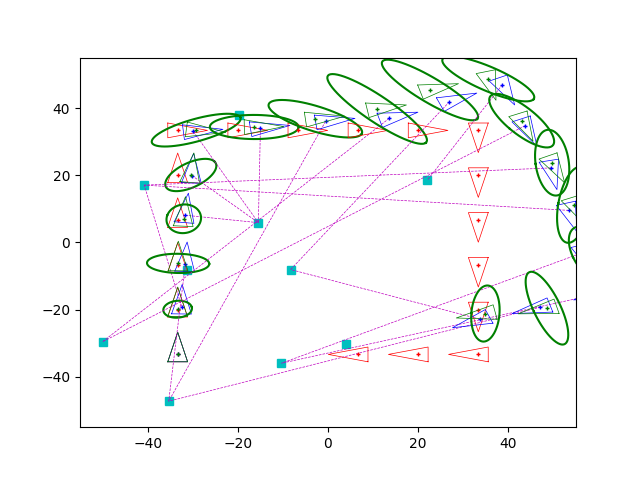
\includegraphics{images/fig5-2-1.png}
\end{figure}
Fig. 1: Execution of the EKF algorithmn for localization, it shows the
true (in blue) and expected (in red) poses, along the results from
localization: pose and ellipse (in green), the existing landmarks (in
cyan), and each observation made (dotted lines).

    \begin{tcolorbox}[breakable, size=fbox, boxrule=1pt, pad at break*=1mm,colback=cellbackground, colframe=cellborder]
\prompt{In}{incolor}{22}{\boxspacing}
\begin{Verbatim}[commandchars=\\\{\}]
\PY{k}{def} \PY{n+nf}{main}\PY{p}{(}\PY{n}{robot}\PY{p}{,}
         \PY{n}{sensor}\PY{p}{,}
         \PY{n}{mode}\PY{o}{=}\PY{l+s+s1}{\PYZsq{}}\PY{l+s+s1}{one\PYZus{}landmark}\PY{l+s+s1}{\PYZsq{}}\PY{p}{,}
         \PY{n}{nSteps}\PY{o}{=}\PY{l+m+mi}{20}\PY{p}{,} \PY{c+c1}{\PYZsh{} Number of motions}
         \PY{n}{turning}\PY{o}{=}\PY{l+m+mi}{5}\PY{p}{,} \PY{c+c1}{\PYZsh{} Number of motions before turning (square path)}
         \PY{n}{Size}\PY{o}{=}\PY{l+m+mf}{50.0}\PY{p}{,}
         \PY{n}{NumLandmarks}\PY{o}{=}\PY{l+m+mi}{10}\PY{p}{)}\PY{p}{:}
    \PY{n}{seed} \PY{o}{=} \PY{l+m+mi}{1}
    \PY{n}{np}\PY{o}{.}\PY{n}{random}\PY{o}{.}\PY{n}{seed}\PY{p}{(}\PY{n}{seed}\PY{p}{)}
    
    \PY{c+c1}{\PYZsh{}Create map}
    \PY{n}{Map}\PY{o}{=}\PY{n}{Size}\PY{o}{*}\PY{l+m+mi}{2}\PY{o}{*}\PY{n}{random}\PY{o}{.}\PY{n}{rand}\PY{p}{(}\PY{l+m+mi}{2}\PY{p}{,}\PY{n}{NumLandmarks}\PY{p}{)}\PY{o}{\PYZhy{}}\PY{n}{Size}
    
    \PY{c+c1}{\PYZsh{} MATPLOTLIB}
    \PY{n}{plt}\PY{o}{.}\PY{n}{ion}\PY{p}{(}\PY{p}{)}
    \PY{n}{fig}\PY{p}{,} \PY{n}{ax} \PY{o}{=} \PY{n}{plt}\PY{o}{.}\PY{n}{subplots}\PY{p}{(}\PY{p}{)}
    \PY{n}{plt}\PY{o}{.}\PY{n}{plot}\PY{p}{(}\PY{n}{Map}\PY{p}{[}\PY{l+m+mi}{0}\PY{p}{,}\PY{p}{:}\PY{p}{]}\PY{p}{,}\PY{n}{Map}\PY{p}{[}\PY{l+m+mi}{1}\PY{p}{,}\PY{p}{:}\PY{p}{]}\PY{p}{,}\PY{l+s+s1}{\PYZsq{}}\PY{l+s+s1}{sc}\PY{l+s+s1}{\PYZsq{}}\PY{p}{)}
    \PY{n}{plt}\PY{o}{.}\PY{n}{axis}\PY{p}{(}\PY{p}{[}\PY{o}{\PYZhy{}}\PY{n}{Size}\PY{o}{\PYZhy{}}\PY{l+m+mi}{15}\PY{p}{,} \PY{n}{Size}\PY{o}{+}\PY{l+m+mi}{15}\PY{p}{,} \PY{o}{\PYZhy{}}\PY{n}{Size}\PY{o}{\PYZhy{}}\PY{l+m+mi}{15}\PY{p}{,} \PY{n}{Size}\PY{o}{+}\PY{l+m+mi}{15}\PY{p}{]}\PY{p}{)}
    
    \PY{n}{robot}\PY{o}{.}\PY{n}{draw}\PY{p}{(}\PY{n}{fig}\PY{p}{,} \PY{n}{ax}\PY{p}{)}
    \PY{n}{fig}\PY{o}{.}\PY{n}{canvas}\PY{o}{.}\PY{n}{draw}\PY{p}{(}\PY{p}{)}
    
    \PY{c+c1}{\PYZsh{} MAIN LOOP}
    
    \PY{n}{u} \PY{o}{=} \PY{n}{np}\PY{o}{.}\PY{n}{vstack}\PY{p}{(}\PY{p}{[}\PY{p}{(}\PY{l+m+mi}{2}\PY{o}{*}\PY{n}{Size}\PY{o}{\PYZhy{}}\PY{l+m+mi}{2}\PY{o}{*}\PY{n}{Size}\PY{o}{/}\PY{l+m+mi}{3}\PY{p}{)}\PY{o}{/}\PY{n}{turning}\PY{p}{,}\PY{l+m+mi}{0}\PY{p}{,}\PY{l+m+mi}{0}\PY{p}{]}\PY{p}{)} \PY{c+c1}{\PYZsh{} control action}
    \PY{n}{plt}\PY{o}{.}\PY{n}{waitforbuttonpress}\PY{p}{(}\PY{o}{\PYZhy{}}\PY{l+m+mi}{1}\PY{p}{)}    
    
    
    \PY{k}{for} \PY{n}{k} \PY{o+ow}{in} \PY{n+nb}{range}\PY{p}{(}\PY{l+m+mi}{0}\PY{p}{,} \PY{n}{nSteps}\PY{o}{\PYZhy{}}\PY{l+m+mi}{3}\PY{p}{)}\PY{p}{:} \PY{c+c1}{\PYZsh{} Main loop}
        \PY{n}{u}\PY{p}{[}\PY{l+m+mi}{2}\PY{p}{]} \PY{o}{=} \PY{l+m+mi}{0}
        \PY{k}{if} \PY{n}{k} \PY{o}{\PYZpc{}} \PY{n}{turning} \PY{o}{==} \PY{n}{turning}\PY{o}{\PYZhy{}}\PY{l+m+mi}{1}\PY{p}{:} \PY{c+c1}{\PYZsh{} Turn?}
            \PY{n}{u}\PY{p}{[}\PY{l+m+mi}{2}\PY{p}{]} \PY{o}{=} \PY{o}{\PYZhy{}}\PY{n}{np}\PY{o}{.}\PY{n}{pi}\PY{o}{/}\PY{l+m+mi}{2}

        \PY{n}{robot}\PY{o}{.}\PY{n}{step}\PY{p}{(}\PY{n}{u}\PY{p}{)}
        
        \PY{c+c1}{\PYZsh{} Get sensor observation/s}
        \PY{k}{if} \PY{n}{mode} \PY{o}{==} \PY{l+s+s1}{\PYZsq{}}\PY{l+s+s1}{one\PYZus{}landmark}\PY{l+s+s1}{\PYZsq{}}\PY{p}{:}
            \PY{c+c1}{\PYZsh{} DONE (Exercise 4)}
            \PY{n}{z}\PY{p}{,} \PY{n}{landmark} \PY{o}{=} \PY{n}{sensor}\PY{o}{.}\PY{n}{random\PYZus{}observation}\PY{p}{(}\PY{n}{robot}\PY{o}{.}\PY{n}{true\PYZus{}pose}\PY{p}{,} \PY{n}{Map}\PY{p}{)}
            \PY{n}{ax}\PY{o}{.}\PY{n}{plot}\PY{p}{(}
                \PY{p}{[}\PY{n}{robot}\PY{o}{.}\PY{n}{true\PYZus{}pose}\PY{p}{[}\PY{l+m+mi}{0}\PY{p}{,}\PY{l+m+mi}{0}\PY{p}{]}\PY{p}{,} \PY{n}{Map}\PY{p}{[}\PY{l+m+mi}{0}\PY{p}{,}\PY{n}{landmark}\PY{p}{]}\PY{p}{]}\PY{p}{,}
                \PY{p}{[}\PY{n}{robot}\PY{o}{.}\PY{n}{true\PYZus{}pose}\PY{p}{[}\PY{l+m+mi}{1}\PY{p}{,}\PY{l+m+mi}{0}\PY{p}{]}\PY{p}{,} \PY{n}{Map}\PY{p}{[}\PY{l+m+mi}{1}\PY{p}{,}\PY{n}{landmark}\PY{p}{]}\PY{p}{]}\PY{p}{,}
                \PY{n}{color}\PY{o}{=}\PY{l+s+s1}{\PYZsq{}}\PY{l+s+s1}{m}\PY{l+s+s1}{\PYZsq{}}\PY{p}{,} \PY{n}{linestyle}\PY{o}{=}\PY{l+s+s2}{\PYZdq{}}\PY{l+s+s2}{\PYZhy{}\PYZhy{}}\PY{l+s+s2}{\PYZdq{}}\PY{p}{,} \PY{n}{linewidth}\PY{o}{=}\PY{o}{.}\PY{l+m+mi}{5}\PY{p}{)}
        \PY{k}{elif} \PY{n}{mode} \PY{o}{==} \PY{l+s+s1}{\PYZsq{}}\PY{l+s+s1}{landmarks\PYZus{}in\PYZus{}fov}\PY{l+s+s1}{\PYZsq{}}\PY{p}{:}
            \PY{c+c1}{\PYZsh{} DONE (Exercise 5)}
            \PY{n}{z}\PY{p}{,} \PY{n}{landmark} \PY{o}{=} \PY{n}{sensor}\PY{o}{.}\PY{n}{observe\PYZus{}in\PYZus{}fov}\PY{p}{(}\PY{n}{robot}\PY{o}{.}\PY{n}{true\PYZus{}pose}\PY{p}{,} \PY{n}{Map}\PY{p}{)}
            \PY{n}{drawObservations}\PY{p}{(}\PY{n}{fig}\PY{p}{,} \PY{n}{ax}\PY{p}{,} \PY{n}{robot}\PY{o}{.}\PY{n}{true\PYZus{}pose}\PY{p}{,} \PY{n}{Map}\PY{p}{[}\PY{p}{:}\PY{p}{,} \PY{n}{landmark}\PY{p}{]}\PY{p}{)}
        
        \PY{n}{robot}\PY{o}{.}\PY{n}{xEst}\PY{p}{,} \PY{n}{robot}\PY{o}{.}\PY{n}{PEst} \PY{o}{=} \PY{n}{EKFLocalization}\PY{p}{(}\PY{n}{robot}\PY{p}{,} \PY{n}{sensor}\PY{p}{,} \PY{n}{u}\PY{p}{,} \PY{n}{z}\PY{p}{,} \PY{n}{landmark}\PY{p}{,} \PY{n}{Map}\PY{p}{)}

        \PY{c+c1}{\PYZsh{} Drawings}
        \PY{c+c1}{\PYZsh{} Plot the FOV of the robot}
        \PY{k}{if} \PY{n}{mode} \PY{o}{==} \PY{l+s+s1}{\PYZsq{}}\PY{l+s+s1}{landmarks\PYZus{}in\PYZus{}fov}\PY{l+s+s1}{\PYZsq{}}\PY{p}{:}
            \PY{n}{h} \PY{o}{=} \PY{n}{sensor}\PY{o}{.}\PY{n}{draw}\PY{p}{(}\PY{n}{fig}\PY{p}{,} \PY{n}{ax}\PY{p}{,} \PY{n}{robot}\PY{o}{.}\PY{n}{true\PYZus{}pose}\PY{p}{)}
        \PY{c+c1}{\PYZsh{}end}

        \PY{n}{robot}\PY{o}{.}\PY{n}{draw}\PY{p}{(}\PY{n}{fig}\PY{p}{,} \PY{n}{ax}\PY{p}{)}

        \PY{n}{fig}\PY{o}{.}\PY{n}{canvas}\PY{o}{.}\PY{n}{draw}\PY{p}{(}\PY{p}{)}
        \PY{n}{plt}\PY{o}{.}\PY{n}{waitforbuttonpress}\PY{p}{(}\PY{o}{\PYZhy{}}\PY{l+m+mi}{1}\PY{p}{)}    

        \PY{k}{if} \PY{n}{mode} \PY{o}{==} \PY{l+s+s1}{\PYZsq{}}\PY{l+s+s1}{landmarks\PYZus{}in\PYZus{}fov}\PY{l+s+s1}{\PYZsq{}}\PY{p}{:}
            \PY{n}{h}\PY{o}{.}\PY{n}{pop}\PY{p}{(}\PY{l+m+mi}{0}\PY{p}{)}\PY{o}{.}\PY{n}{remove}\PY{p}{(}\PY{p}{)}
        \PY{n}{fig}\PY{o}{.}\PY{n}{canvas}\PY{o}{.}\PY{n}{draw}\PY{p}{(}\PY{p}{)}
\end{Verbatim}
\end{tcolorbox}

    \begin{tcolorbox}[breakable, size=fbox, boxrule=1pt, pad at break*=1mm,colback=cellbackground, colframe=cellborder]
\prompt{In}{incolor}{25}{\boxspacing}
\begin{Verbatim}[commandchars=\\\{\}]
\PY{c+c1}{\PYZsh{} RUN}
\PY{n}{mode} \PY{o}{=} \PY{l+s+s1}{\PYZsq{}}\PY{l+s+s1}{one\PYZus{}landmark}\PY{l+s+s1}{\PYZsq{}}
\PY{c+c1}{\PYZsh{}mode = \PYZsq{}landmarks\PYZus{}in\PYZus{}fov\PYZsq{}}

\PY{n}{Size}\PY{o}{=}\PY{l+m+mf}{50.0}

\PY{c+c1}{\PYZsh{} Robot base characterization}
\PY{n}{SigmaX} \PY{o}{=} \PY{l+m+mf}{0.8} \PY{c+c1}{\PYZsh{} Standard deviation in the x axis}
\PY{n}{SigmaY} \PY{o}{=} \PY{l+m+mf}{0.8} \PY{c+c1}{\PYZsh{} Standard deviation in the y axis}
\PY{n}{SigmaTheta} \PY{o}{=} \PY{l+m+mf}{0.1} \PY{c+c1}{\PYZsh{} Bearing standar deviation}
\PY{n}{R} \PY{o}{=} \PY{n}{np}\PY{o}{.}\PY{n}{diag}\PY{p}{(}\PY{p}{[}\PY{n}{SigmaX}\PY{o}{*}\PY{o}{*}\PY{l+m+mi}{2}\PY{p}{,} \PY{n}{SigmaY}\PY{o}{*}\PY{o}{*}\PY{l+m+mi}{2}\PY{p}{,} \PY{n}{SigmaTheta}\PY{o}{*}\PY{o}{*}\PY{l+m+mi}{2}\PY{p}{]}\PY{p}{)} \PY{c+c1}{\PYZsh{} Cov matrix}

\PY{n}{true\PYZus{}pose} \PY{o}{=} \PY{n}{np}\PY{o}{.}\PY{n}{vstack}\PY{p}{(}\PY{p}{[}\PY{o}{\PYZhy{}}\PY{n}{Size}\PY{o}{+}\PY{n}{Size}\PY{o}{/}\PY{l+m+mi}{3}\PY{p}{,} \PY{o}{\PYZhy{}}\PY{n}{Size}\PY{o}{+}\PY{n}{Size}\PY{o}{/}\PY{l+m+mi}{3}\PY{p}{,} \PY{n}{np}\PY{o}{.}\PY{n}{pi}\PY{o}{/}\PY{l+m+mi}{2}\PY{p}{]}\PY{p}{)}
\PY{n}{robot} \PY{o}{=} \PY{n}{Robot}\PY{p}{(}\PY{n}{true\PYZus{}pose}\PY{p}{,} \PY{n}{R}\PY{p}{)}

\PY{c+c1}{\PYZsh{} Sensor characterization}
\PY{n}{SigmaR} \PY{o}{=} \PY{l+m+mi}{1} \PY{c+c1}{\PYZsh{} Standard deviation of the range}
\PY{n}{SigmaB} \PY{o}{=} \PY{l+m+mf}{0.7} \PY{c+c1}{\PYZsh{} Standard deviation of the bearing}
\PY{n}{Q} \PY{o}{=} \PY{n}{np}\PY{o}{.}\PY{n}{diag}\PY{p}{(}\PY{p}{[}\PY{n}{SigmaR}\PY{o}{*}\PY{o}{*}\PY{l+m+mi}{2}\PY{p}{,} \PY{n}{SigmaB}\PY{o}{*}\PY{o}{*}\PY{l+m+mi}{2}\PY{p}{]}\PY{p}{)} \PY{c+c1}{\PYZsh{} Cov matrix}

\PY{n}{sensor} \PY{o}{=} \PY{n}{Sensor}\PY{p}{(}\PY{n}{Q}\PY{p}{)}

\PY{n}{main}\PY{p}{(}\PY{n}{robot}\PY{p}{,} \PY{n}{sensor}\PY{p}{,} \PY{n}{mode}\PY{o}{=}\PY{n}{mode}\PY{p}{,} \PY{n}{Size}\PY{o}{=}\PY{n}{Size}\PY{p}{)}
\end{Verbatim}
\end{tcolorbox}


\begin{figure}
\centering
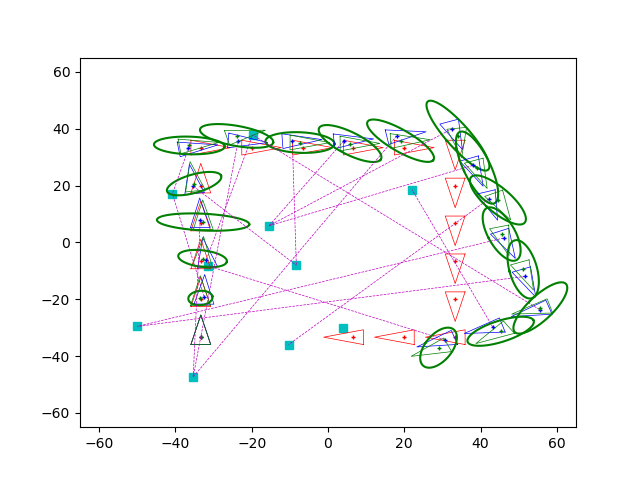
\includegraphics{images/salidaAssignment4.png}
\end{figure}

    \hypertarget{assignment-5-implementing-the-fov-of-a-sensor.}{%
\subsubsection{\texorpdfstring{\textbf{{ASSIGNMENT 5: Implementing the
FoV of a
sensor.}}}{ASSIGNMENT 5: Implementing the FoV of a sensor.}}\label{assignment-5-implementing-the-fov-of-a-sensor.}}

Sensors exhibit certain physical limitations regarding their field of
view (FoV) and maximum operating distance (max. Range). Besides, these
devices often do not deliver measurmenets from just one landmark each
time, but from all those landmarks in the FoV.

The \texttt{FOVSensor()} class below extends the \texttt{Sensor()} one
to implement this behaviour. Complete the \texttt{observe\_in\_fov()}
method to consider that the sensor can only provide information from the
landmkars in a limited range \(r_l\) and a limited orientation
\(\pm \alpha\) with respect to the robot pose. For that:

\begin{enumerate}
\def\labelenumi{\arabic{enumi}.}
\tightlist
\item
  Get the observations to every landmark in the map. Use the
  \texttt{observe()} function previously implemented for that, but with
  the argument \texttt{flatten=False}. With that option the function
  returns the measurements as: \[
  z = \begin{bmatrix} d_1 &  \cdots &  d_m \\ \theta_1 & \cdots & \theta_m \end{bmatrix}
  \]
\item
  Check which observations lay in the sensor FoV and maximum operating
  distance. \emph{Hint: for that, you can use the
  \href{https://docs.scipy.org/doc/numpy/reference/generated/numpy.asarray.html}{\texttt{np.asarray()}}
  function with the conditions to be fulfilled by the valid measurements
  inside, and then filter the results with
  \href{https://docs.scipy.org/doc/numpy/reference/generated/numpy.nonzero.html}{\texttt{np.nonzero()}}}.
\item
  Flatten the resultant matrix \texttt{z} to be again a vector, so it
  has the shape \((2 \times \#Observed\_landmarks,1)\). \emph{Hint: take
  a look at
  \href{https://docs.scipy.org/doc/numpy/reference/generated/numpy.ndarray.flatten.html}{\texttt{np.ndarray.flatten()}}
  and choose the proper argument.}
\end{enumerate}

Notice that it could happen that any landmark exists in the field of
view of the sensor, so the robot couldn't gather sensory information in
that iteration. This, which is a problem using Least Squares
Positioning, is not an issue with EKF. \textbf{\emph{Hint: you can
change the value of \texttt{seed} within the \texttt{main()}function to
try different executions.}}

    \begin{tcolorbox}[breakable, size=fbox, boxrule=1pt, pad at break*=1mm,colback=cellbackground, colframe=cellborder]
\prompt{In}{incolor}{26}{\boxspacing}
\begin{Verbatim}[commandchars=\\\{\}]
\PY{k}{class} \PY{n+nc}{FOVSensor}\PY{p}{(}\PY{n}{Sensor}\PY{p}{)}\PY{p}{:}
    \PY{k}{def} \PY{n+nf+fm}{\PYZus{}\PYZus{}init\PYZus{}\PYZus{}}\PY{p}{(}\PY{n+nb+bp}{self}\PY{p}{,} \PY{n}{cov}\PY{p}{,} \PY{n}{fov}\PY{p}{,} \PY{n}{max\PYZus{}range}\PY{p}{)}\PY{p}{:}
        \PY{n+nb}{super}\PY{p}{(}\PY{p}{)}\PY{o}{.}\PY{n+nf+fm}{\PYZus{}\PYZus{}init\PYZus{}\PYZus{}}\PY{p}{(}\PY{n}{cov}\PY{p}{)}
        \PY{n+nb+bp}{self}\PY{o}{.}\PY{n}{fov} \PY{o}{=} \PY{n}{fov}
        \PY{n+nb+bp}{self}\PY{o}{.}\PY{n}{max\PYZus{}range} \PY{o}{=} \PY{n}{max\PYZus{}range}
    
    \PY{k}{def} \PY{n+nf}{observe\PYZus{}in\PYZus{}fov}\PY{p}{(}\PY{n+nb+bp}{self}\PY{p}{,} \PY{n}{from\PYZus{}pose}\PY{p}{,} \PY{n}{world}\PY{p}{,} \PY{n}{noisy}\PY{o}{=}\PY{k+kc}{True}\PY{p}{)}\PY{p}{:}
        \PY{l+s+sd}{\PYZdq{}\PYZdq{}\PYZdq{} Get all observations in the fov}

\PY{l+s+sd}{        Args:}
\PY{l+s+sd}{            from\PYZus{}pose: Position(real) of the robot which takes the observation}
\PY{l+s+sd}{            world: List of world coordinates of some landmarks}
\PY{l+s+sd}{            noisy: Flag, if true then add noise (Exercise 2)}

\PY{l+s+sd}{        Returns:}
\PY{l+s+sd}{            Numpy array of polar coordinates of landmarks from the perspective of our robot}
\PY{l+s+sd}{            They are organised in a vertical vector ls = [d\PYZus{}0 , a\PYZus{}0, d\PYZus{}1, ..., a\PYZus{}n]\PYZsq{}}
\PY{l+s+sd}{            Dims (2*n\PYZus{}landmarks, 1) }
\PY{l+s+sd}{        \PYZdq{}\PYZdq{}\PYZdq{}}                
        \PY{c+c1}{\PYZsh{} 1. Get observations to every landmark in the map WITHOUT NOISE}
        \PY{n}{z} \PY{o}{=} \PY{n+nb+bp}{self}\PY{o}{.}\PY{n}{observe}\PY{p}{(}\PY{n}{from\PYZus{}pose}\PY{p}{,} \PY{n}{world}\PY{p}{,} \PY{k+kc}{False}\PY{p}{,} \PY{k+kc}{False}\PY{p}{)}
        
        \PY{c+c1}{\PYZsh{} 2. Check which ones lay on the sensor FOV}
        \PY{n}{angle\PYZus{}limit} \PY{o}{=} \PY{n+nb+bp}{self}\PY{o}{.}\PY{n}{fov}\PY{o}{/}\PY{l+m+mi}{2} \PY{c+c1}{\PYZsh{} auxiliar variable}
        \PY{n}{t} \PY{o}{=} \PY{n}{np}\PY{o}{.}\PY{n}{asarray}\PY{p}{(}\PY{n}{z}\PY{p}{[}\PY{l+m+mi}{0}\PY{p}{]} \PY{o}{\PYZlt{}} \PY{n+nb+bp}{self}\PY{o}{.}\PY{n}{max\PYZus{}range}\PY{p}{)}
        \PY{n}{t}\PY{p}{[}\PY{n}{np}\PY{o}{.}\PY{n}{asarray}  \PY{p}{(}\PY{n}{z}\PY{p}{[}\PY{l+m+mi}{1}\PY{p}{]} \PY{o}{\PYZgt{}} \PY{n}{angle\PYZus{}limit}\PY{p}{)}\PY{p}{]} \PY{o}{=} \PY{k+kc}{False}
        \PY{n}{feats\PYZus{}idx} \PY{o}{=} \PY{n}{t} \PY{c+c1}{\PYZsh{} indices of the valid observations    }
                
        \PY{k}{if} \PY{n}{noisy}\PY{p}{:}
            \PY{c+c1}{\PYZsh{} 1. Get observations to every landmark in the map WITH NOISE}
            \PY{n}{z} \PY{o}{=} \PY{n+nb+bp}{self}\PY{o}{.}\PY{n}{observe}\PY{p}{(}\PY{n}{from\PYZus{}pose}\PY{p}{,} \PY{n}{world}\PY{p}{,} \PY{k+kc}{True}\PY{p}{,} \PY{k+kc}{False}\PY{p}{)}
            
        \PY{n}{z} \PY{o}{=} \PY{n}{z}\PY{p}{[}\PY{p}{:}\PY{p}{,} \PY{n}{feats\PYZus{}idx}\PY{p}{]} \PY{c+c1}{\PYZsh{} extracts the valid observations from z \PYZsh{} PROBLEMA AQUI}
               
        \PY{c+c1}{\PYZsh{} 3. Flatten the  resultant vector of measurements so z=[d\PYZus{}1,theta\PYZus{}1,d\PYZus{}2,theta\PYZus{}2,...,d\PYZus{}n,theta\PYZus{}n]   }
        \PY{k}{if} \PY{n}{z}\PY{o}{.}\PY{n}{size}\PY{o}{\PYZgt{}}\PY{l+m+mi}{0}\PY{p}{:}
            \PY{n}{z} \PY{o}{=} \PY{n}{np}\PY{o}{.}\PY{n}{vstack}\PY{p}{(}\PY{n}{z}\PY{o}{.}\PY{n}{flatten}\PY{p}{(}\PY{l+s+s1}{\PYZsq{}}\PY{l+s+s1}{F}\PY{l+s+s1}{\PYZsq{}}\PY{p}{)}\PY{p}{)}
            
        \PY{k}{return} \PY{n}{z}\PY{p}{,} \PY{n}{feats\PYZus{}idx}
    
    \PY{k}{def} \PY{n+nf}{draw}\PY{p}{(}\PY{n+nb+bp}{self}\PY{p}{,} \PY{n}{fig}\PY{p}{,} \PY{n}{ax}\PY{p}{,} \PY{n}{from\PYZus{}pose}\PY{p}{)}\PY{p}{:}
        \PY{l+s+sd}{\PYZdq{}\PYZdq{}\PYZdq{} Draws the Field of View of the sensor from the robot pose \PYZdq{}\PYZdq{}\PYZdq{}}
        \PY{k}{return} \PY{n}{drawFOV}\PY{p}{(}\PY{n}{fig}\PY{p}{,} \PY{n}{ax}\PY{p}{,} \PY{n}{from\PYZus{}pose}\PY{p}{,} \PY{n+nb+bp}{self}\PY{o}{.}\PY{n}{fov}\PY{p}{,} \PY{n+nb+bp}{self}\PY{o}{.}\PY{n}{max\PYZus{}range}\PY{p}{)}   
\end{Verbatim}
\end{tcolorbox}

    You can now \textbf{try} your new and more realistic sensor.

    \begin{tcolorbox}[breakable, size=fbox, boxrule=1pt, pad at break*=1mm,colback=cellbackground, colframe=cellborder]
\prompt{In}{incolor}{27}{\boxspacing}
\begin{Verbatim}[commandchars=\\\{\}]
\PY{c+c1}{\PYZsh{} TRY IT!}
\PY{n}{np}\PY{o}{.}\PY{n}{random}\PY{o}{.}\PY{n}{seed}\PY{p}{(}\PY{l+m+mi}{0}\PY{p}{)}

\PY{c+c1}{\PYZsh{} Create the sensor object}
\PY{n}{cov} \PY{o}{=} \PY{n}{np}\PY{o}{.}\PY{n}{diag}\PY{p}{(}\PY{p}{[}\PY{l+m+mf}{0.1}\PY{o}{*}\PY{o}{*}\PY{l+m+mi}{2}\PY{p}{,} \PY{l+m+mf}{0.1}\PY{o}{*}\PY{o}{*}\PY{l+m+mi}{2}\PY{p}{]}\PY{p}{)} \PY{c+c1}{\PYZsh{} Cov matrix}
\PY{n}{fov} \PY{o}{=} \PY{n}{np}\PY{o}{.}\PY{n}{pi}\PY{o}{/}\PY{l+m+mi}{2}
\PY{n}{max\PYZus{}range} \PY{o}{=} \PY{l+m+mi}{2}
\PY{n}{sensor} \PY{o}{=} \PY{n}{FOVSensor}\PY{p}{(}\PY{n}{cov}\PY{p}{,} \PY{n}{fov}\PY{p}{,} \PY{n}{max\PYZus{}range}\PY{p}{)}

\PY{c+c1}{\PYZsh{} Create a map with three landmarks}
\PY{n}{Map} \PY{o}{=} \PY{n}{np}\PY{o}{.}\PY{n}{array}\PY{p}{(}\PY{p}{[}\PY{p}{[}\PY{l+m+mf}{2.}\PY{p}{,} \PY{l+m+mf}{2.5}\PY{p}{,} \PY{l+m+mf}{3.5}\PY{p}{,} \PY{l+m+mf}{0.5}\PY{p}{]}\PY{p}{,}\PY{p}{[}\PY{l+m+mf}{2.}\PY{p}{,} \PY{l+m+mf}{3.}\PY{p}{,} \PY{l+m+mf}{1.5}\PY{p}{,} \PY{l+m+mf}{3.5}\PY{p}{]}\PY{p}{]}\PY{p}{)}

\PY{c+c1}{\PYZsh{} Take an observation of landmarks in FoV}
\PY{n}{robot\PYZus{}pose} \PY{o}{=} \PY{n}{np}\PY{o}{.}\PY{n}{vstack}\PY{p}{(}\PY{p}{[}\PY{l+m+mf}{1.}\PY{p}{,}\PY{l+m+mf}{2.}\PY{p}{,}\PY{l+m+mf}{0.}\PY{p}{]}\PY{p}{)}
\PY{n}{z}\PY{p}{,} \PY{n}{feats\PYZus{}idx} \PY{o}{=} \PY{n}{sensor}\PY{o}{.}\PY{n}{observe\PYZus{}in\PYZus{}fov}\PY{p}{(}\PY{n}{robot\PYZus{}pose}\PY{p}{,} \PY{n}{Map}\PY{p}{)}

\PY{n+nb}{print}\PY{p}{(}\PY{l+s+s1}{\PYZsq{}}\PY{l+s+s1}{z:}\PY{l+s+s1}{\PYZsq{}} \PY{o}{+}\PY{n+nb}{str}\PY{p}{(}\PY{n}{z}\PY{p}{)}\PY{p}{)}


\PY{c+c1}{\PYZsh{} Plot results}
\PY{n}{fig}\PY{p}{,} \PY{n}{ax} \PY{o}{=} \PY{n}{plt}\PY{o}{.}\PY{n}{subplots}\PY{p}{(}\PY{p}{)}
\PY{n}{plt}\PY{o}{.}\PY{n}{axis}\PY{p}{(}\PY{p}{[}\PY{l+m+mi}{0}\PY{p}{,} \PY{l+m+mi}{5}\PY{p}{,} \PY{l+m+mi}{0}\PY{p}{,} \PY{l+m+mi}{5}\PY{p}{]}\PY{p}{)}
\PY{n}{plt}\PY{o}{.}\PY{n}{title}\PY{p}{(}\PY{l+s+s1}{\PYZsq{}}\PY{l+s+s1}{Measuremets to landmarks in sensor FOV}\PY{l+s+s1}{\PYZsq{}}\PY{p}{)}
\PY{n}{plt}\PY{o}{.}\PY{n}{plot}\PY{p}{(}\PY{n}{Map}\PY{p}{[}\PY{l+m+mi}{0}\PY{p}{,}\PY{p}{:}\PY{p}{]}\PY{p}{,}\PY{n}{Map}\PY{p}{[}\PY{l+m+mi}{1}\PY{p}{,}\PY{p}{:}\PY{p}{]}\PY{p}{,}\PY{l+s+s1}{\PYZsq{}}\PY{l+s+s1}{sc}\PY{l+s+s1}{\PYZsq{}}\PY{p}{)}
\PY{n}{sensor}\PY{o}{.}\PY{n}{draw}\PY{p}{(}\PY{n}{fig}\PY{p}{,} \PY{n}{ax}\PY{p}{,} \PY{n}{robot\PYZus{}pose}\PY{p}{)}
\PY{n}{drawObservations}\PY{p}{(}\PY{n}{fig}\PY{p}{,} \PY{n}{ax}\PY{p}{,} \PY{n}{robot\PYZus{}pose}\PY{p}{,} \PY{n}{Map}\PY{p}{[}\PY{p}{:}\PY{p}{,} \PY{n}{feats\PYZus{}idx}\PY{p}{]}\PY{p}{)}
\PY{n}{DrawRobot}\PY{p}{(}\PY{n}{fig}\PY{p}{,}\PY{n}{ax}\PY{p}{,}\PY{n}{robot\PYZus{}pose}\PY{p}{)}
\end{Verbatim}
\end{tcolorbox}

    \begin{Verbatim}[commandchars=\\\{\}]
z:[[1.17640523]
 [0.1867558 ]
 [1.84279136]
 [0.49027482]]
    \end{Verbatim}

    {Expected output:}

\begin{verbatim}
z:[[1.17640523]
 [0.1867558 ]
 [1.84279136]
 [0.49027482]]
\end{verbatim}

    \hypertarget{playing-with-ekf-and-the-new-sensor}{%
\subsection{Playing with EKF and the new
sensor}\label{playing-with-ekf-and-the-new-sensor}}

And finally, play with your own FULL implementation of the EKF filter
with a more realistic sensor :)

\textbf{Example}

The figure below shows an example of the execution of EKF using
information from all the landmarks within the FOV:

\begin{figure}
\centering
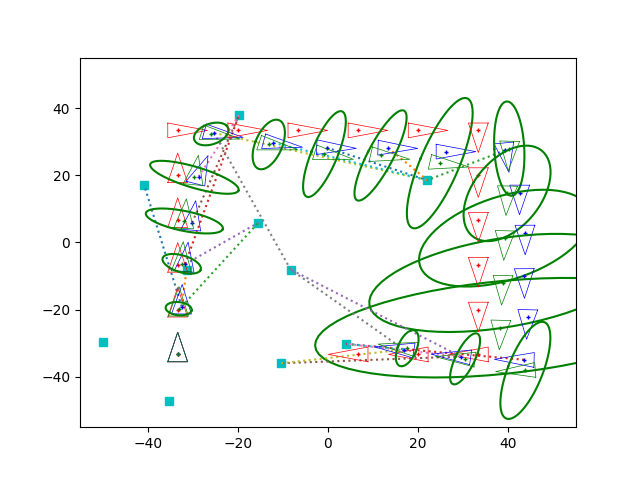
\includegraphics{images/fig5-2-2.png}
\end{figure}
Fig. 2: Execution of the EKF algorithmn for localization. Same as in
Fig. 1, except now our robot can observe every lanmark in its f.o.v.

    \begin{tcolorbox}[breakable, size=fbox, boxrule=1pt, pad at break*=1mm,colback=cellbackground, colframe=cellborder]
\prompt{In}{incolor}{13}{\boxspacing}
\begin{Verbatim}[commandchars=\\\{\}]
\PY{c+c1}{\PYZsh{} RUN}
\PY{c+c1}{\PYZsh{}mode = \PYZsq{}one\PYZus{}landmark\PYZsq{}}
\PY{n}{mode} \PY{o}{=} \PY{l+s+s1}{\PYZsq{}}\PY{l+s+s1}{landmarks\PYZus{}in\PYZus{}fov}\PY{l+s+s1}{\PYZsq{}}
\PY{n}{Size}\PY{o}{=}\PY{l+m+mf}{50.0}

\PY{c+c1}{\PYZsh{} Robot base characterization}
\PY{n}{SigmaX} \PY{o}{=} \PY{l+m+mf}{0.8} \PY{c+c1}{\PYZsh{} Standard deviation in the x axis}
\PY{n}{SigmaY} \PY{o}{=} \PY{l+m+mf}{0.8} \PY{c+c1}{\PYZsh{} Standard deviation in the y axis}
\PY{n}{SigmaTheta} \PY{o}{=} \PY{l+m+mf}{0.1} \PY{c+c1}{\PYZsh{} Bearing standar deviation}
\PY{n}{R} \PY{o}{=} \PY{n}{np}\PY{o}{.}\PY{n}{diag}\PY{p}{(}\PY{p}{[}\PY{n}{SigmaX}\PY{o}{*}\PY{o}{*}\PY{l+m+mi}{2}\PY{p}{,} \PY{n}{SigmaY}\PY{o}{*}\PY{o}{*}\PY{l+m+mi}{2}\PY{p}{,} \PY{n}{SigmaTheta}\PY{o}{*}\PY{o}{*}\PY{l+m+mi}{2}\PY{p}{]}\PY{p}{)} \PY{c+c1}{\PYZsh{} Cov matrix}

\PY{n}{true\PYZus{}pose} \PY{o}{=} \PY{n}{np}\PY{o}{.}\PY{n}{vstack}\PY{p}{(}\PY{p}{[}\PY{o}{\PYZhy{}}\PY{n}{Size}\PY{o}{+}\PY{n}{Size}\PY{o}{/}\PY{l+m+mi}{3}\PY{p}{,} \PY{o}{\PYZhy{}}\PY{n}{Size}\PY{o}{+}\PY{n}{Size}\PY{o}{/}\PY{l+m+mi}{3}\PY{p}{,} \PY{n}{np}\PY{o}{.}\PY{n}{pi}\PY{o}{/}\PY{l+m+mi}{2}\PY{p}{]}\PY{p}{)}
\PY{n}{robot} \PY{o}{=} \PY{n}{Robot}\PY{p}{(}\PY{n}{true\PYZus{}pose}\PY{p}{,} \PY{n}{R}\PY{p}{)}

\PY{c+c1}{\PYZsh{} Sensor characterization}
\PY{n}{SigmaR} \PY{o}{=} \PY{l+m+mi}{1} \PY{c+c1}{\PYZsh{} Standard deviation of the range}
\PY{n}{SigmaB} \PY{o}{=} \PY{l+m+mf}{0.7} \PY{c+c1}{\PYZsh{} Standard deviation of the bearing}
\PY{n}{Q} \PY{o}{=} \PY{n}{np}\PY{o}{.}\PY{n}{diag}\PY{p}{(}\PY{p}{[}\PY{n}{SigmaR}\PY{o}{*}\PY{o}{*}\PY{l+m+mi}{2}\PY{p}{,} \PY{n}{SigmaB}\PY{o}{*}\PY{o}{*}\PY{l+m+mi}{2}\PY{p}{]}\PY{p}{)} \PY{c+c1}{\PYZsh{} Cov matrix}
\PY{n}{fov} \PY{o}{=} \PY{n}{np}\PY{o}{.}\PY{n}{pi}\PY{o}{/}\PY{l+m+mi}{2} \PY{c+c1}{\PYZsh{} field of view = 2*alpha}
\PY{n}{max\PYZus{}range} \PY{o}{=} \PY{n}{Size} \PY{c+c1}{\PYZsh{} maximum sensor measurement range}

\PY{n}{sensor} \PY{o}{=} \PY{n}{FOVSensor}\PY{p}{(}\PY{n}{Q}\PY{p}{,} \PY{n}{fov}\PY{p}{,} \PY{n}{max\PYZus{}range}\PY{p}{)}

\PY{n}{main}\PY{p}{(}\PY{n}{robot}\PY{p}{,} \PY{n}{sensor}\PY{p}{,} \PY{n}{mode}\PY{o}{=}\PY{n}{mode}\PY{p}{,} \PY{n}{Size}\PY{o}{=}\PY{n}{Size}\PY{p}{)}
\end{Verbatim}
\end{tcolorbox}

    \hypertarget{thinking-about-it-1}{%
\subsubsection{Thinking about it (1)}\label{thinking-about-it-1}}

Having completed the EKF implementation, you are ready to \textbf{answer
the following questions}:

\begin{itemize}
\item
  What are the dimensions of the Jacobians of the observation model
  (matrix H)? Why?

  2*numLandmarks x 3. Becaruse each landmark has 2 variables, X and Y,
  and poses have 3 variables, X, Y and Angle
\item
  Discuss the evolution of the ideal, true and estimated poses when
  executing the EKF filter (with the initial sensor).

  The ideal pose is always where the robot is supposed to be when it
  moves. The true pose is the pose where the robot is after the
  movement, applying some noise to the movement. The estimated pose is
  the pose that calculates the robot measuring the distance to landmark
  and calculating his pose using EKF filter.
\item
  Discuss the evolution of the ideal, true and estimated poses when
  executing the EKF filter (with the sensor implementing a FOV). Pay
  special attention to their associated uncertainties.

  It would be the same only that when correcting the predicted position,
  it may not reduce the uncertainty depending on whether the robot is
  capable to observe landmarks or not. The more landmarks observed, more
  reduced will be the uncertainty.
\item
  What happens in the EKF filter when the robot performs a motion
  command, but it is unable to measure distances to any landmark,
  i.e.~they are out of the sensor FOV?

  As I said in the las answer, the model in the correction step will not
  able to reduce the uncertainty.
\end{itemize}


    % Add a bibliography block to the postdoc
    
    
    
\end{document}
